% Use only LaTeX2e, calling the article.cls class and 12-point type.

\documentclass[12pt]{article}

% Users of the {thebibliography} environment or BibTeX should use the
% scicite.sty package, downloadable from *Science* at
% http://www.sciencemag.org/authors/preparing-manuscripts-using-latex 
% This package should properly format in-text
% reference calls and reference-list numbers.

\usepackage{scicite}

\usepackage{times}

%ONES I ADDED
\usepackage{graphicx} %Package for adding figures
\usepackage{authblk}
\usepackage{url} % for easy url hyperlinks
\usepackage{amsmath,amssymb}

\DeclareMathOperator{\E}{\mathbb{E}}

% The preamble here sets up a lot of new/revised commands and
% environments.  It's annoying, but please do *not* try to strip these
% out into a separate .sty file (which could lead to the loss of some
% information when we convert the file to other formats).  Instead, keep
% them in the preamble of your main LaTeX source file.


% The following parameters seem to provide a reasonable page setup.

\topmargin 0.0cm
\oddsidemargin 0.2cm
\textwidth 16cm 
\textheight 21cm
\footskip 1.0cm


%The next command sets up an environment for the abstract to your paper.

\newenvironment{sciabstract}{%
\begin{quote} \bf}
{\end{quote}}


% Include your paper's title here

\title{Non-linear dynamics drive a mass invariant evolutionary stable strategy in predator-prey systems} 


% Place the author information here.  Please hand-code the contact
% information and notecalls; do *not* use \footnote commands.  Let the
% author contact information appear immediately below the author names
% as shown.  We would also prefer that you don't change the type-size
% settings shown here.

\author[1]{Michael J. Noonan$^\ast$}
\affil[1]{\small The University of British Columbia Okanagan, Kelowna, BC, Canada}

\author[2]{Ricardo Martinez-Garcia}
\affil[2]{\small ICTP South American Institute for Fundamental Research \& Instituto de Física Teórica, Universidade Estadual Paulista - UNESP, Rua Dr. Bento Teobaldo Ferraz 271, Bloco 2 - Barra Funda, 01140-070 São Paulo, SP, Brazil}

\author[3,4]{C. H. Fleming}
\affil[3]{\small University of Maryland College Park, College Park, MD, USA}
\affil[4]{\small Smithsonian Conservation Biology Institute, Front Royal, VA, USA}

\author[2]{Benjamin Garcia De Figueiredo}
\affil[2]{\small ICTP South American Institute for Fundamental Research \& Instituto de Física Teórica, Universidade Estadual Paulista - UNESP, Rua Dr. Bento Teobaldo Ferraz 271, Bloco 2 - Barra Funda, 01140-070 São Paulo, SP, Brazil}

\author[]{DATA PROVIDERS}

\author[5,6,7]{Justin M. Calabrese}
\affil[5]{Center for Advanced Systems Understanding (CASUS), Görlitz, Germany}
\affil[6]{Helmholtz-Zentrum Dresden-Rossendorf (HZDR), Dresden, Germany}
\affil[7]{Department of Biology, University of Maryland, College Park, MD, USA}

%\author
%{Michael J. Noonan,$^{1\ast}$, Ricardo Martinez-Garcia,$^{2 \ast}$ Christen H. Fleming,$^{1,2}$, DATA PROVIDERS, Justin M. Calabrese$^{1,2}$\\
%\\
%\normalsize{$^{1}$The University of British Columbia Okanagan, Kelowna, BC, Canada}\\
%\normalsize{$^{2}$Smithsonian Conservation Biology Institute, National Zoological Park,}\\
%\normalsize{$^{3}$Smithsonian Conservation Biology Institute, National Zoological Park,}\\
%\normalsize{1500 Remount Rd., Front Royal, VA 22630, USA}\\
%\normalsize{$^{4}$Department of Biology, University of Maryland, College Park, MD 20742, USA}\\
%\\
%\normalsize{$^\ast$To whom correspondence should be addressed; E-mail:  NoonanM@si.edu.}
%}

% Include the date command, but leave its argument blank.

\date{}



%%%%%%%%%%%%%%%%% END OF PREAMBLE %%%%%%%%%%%%%%%%



\begin{document} 

% Double-space the manuscript.

\baselineskip24pt

% Make the title.

\maketitle 



% Place your abstract within the special {sciabstract} environment.

\begin{sciabstract}
Abstract goes here.
\end{sciabstract}



% In setting up this template for *Science* papers, we've used both
% the \section* command and the \paragraph* command for topical
% divisions.  Which you use will of course depend on the type of paper
% you're writing.  Review Articles tend to have displayed headings, for
% which \section* is more appropriate; Research Articles, when they have
% formal topical divisions at all, tend to signal them with bold text
% that runs into the paragraph, for which \paragraph* is the right
% choice.  Either way, use the asterisk (*) modifier, as shown, to
% suppress numbering.

\section*{Introduction}

%The metabolic theory of ecology \cite{Kleiber:1947,West:1997, McNab:2002wf, Brown:2004} suggests that body mass is a `super trait' that governs most observed biological patterns from the scale of the individual to the ecosystem \cite{Enquist:2003}. This theory has led to the formulation of numerous body size scaling rules. Prime among these is the relationship between body mass and animal space use, an allometry that has guided ecological theory for more than 50 years \cite{McNab:1963,CalderIII:1983bh,Grant:1992kn,Jetz:2004er,Tamburello:2015}. Assuming that energetic requirements are determined by the whole-organism field metabolic rate \cite{Kleiber:1947}, home range area, $H$, should scale positively with body mass, $M$, as $H = B_{0}M^b$, where $B_{0}$ is a normalization constant and $b$ the scaling exponent \cite{McNab:1963}. However, despite decades of research focused on identifying the scaling exponent of this relationship \cite{McNab:1963, CalderIII:1983bh, Grant:1992kn,Kelt:2001,Jetz:2004er,Tucker:2014,Tamburello:2015}, there has been no attention on how movement within home range areas scales across taxa.

%The metabolic theory of ecology suggests that body mass is a `super trait' that governs most observed biological patterns from the scale of the individual to the ecosystem \cite{Kleiber:1947,West:1997, McNab:2002wf, Enquist:2003,Brown:2004}. Assuming that energetic requirements are determined by the whole-organism field metabolic rate \cite{Kleiber:1947}, and that one of the principal reasons why animals move is to increase the rate at which food is encountered \cite{Charnov:1976wz,Rosenzweig:1981,Turchin:2003,DeKnegt:2007bg,Barraquand:2013}, the expectation is that home range area should scale positively with body mass. Indeed, the positive allometry between home-range area and body mass has received unequivocal support from more than 50 years of research into animal movement \cite{McNab:1963,CalderIII:1983bh,Jetz:2004er,Tamburello:2015,Noonan:2020}. However, what is less understood is how predator-prey dynamics play out across the mass spectrum. Unsurprisingly, more than 50 years of research have demonstrated the animal movement and space use are strongly tied to body size \cite{McNab:1963,CalderIII:1983bh,Grant:1992kn,Jetz:2004er,Visser:2006,Tamburello:2015,Hirt:2017}. 

For motile species, movement represents a key mechanistic link between individual behaviour and higher-level ecological processes \cite{Holling:1959,Kareiva:1987,Huston:1988,Turchin:1998td,Barraquand:2013,Spiegel:2017be,Dougherty:2018}. Because of the evolutionary significance of optimal foraging theory \cite{Charnov:1976wz,Pyke:1984,DeKnegt:2007bg,Fagan:2013gx} and predator-prey dynamics \cite{Volterra:1928,Elton:1942,Mitchell:2002en,Fortin:2005fj,Barraquand:2013}, there should be strong selection pressure on any movement strategies that optimize encounter rates. In this respect, directed (i.e., ballistic) movement leads to higher encounter rates, whereas more tortuous (i.e., diffusive) movement tends to decrease encounter rates \cite{Gerritsen:1977,Visser:2006,Hutchinson:2007,Bartumeus:2008,Gurarie:2011ic}. Therefore, to maximize the rate at which prey are encountered, predatory species should be expected to exhibit more ballistic motion than their prey species. Conversely, for herbivores feeding on immobile, widely available vegetation, mortality due to predation is a major evolutionary force \cite{McNaughton:1986, Reale:2003, Sinclair:2003}. Compared to predatory species therefore, we would expect herbivorous prey species to maintain relatively diffusive movement in order to minimize the rate at which they encounter potential predators. Although the importance of ballistic motion in determining encounter rates is well recognized \cite{Visser:2006, Bartumeus:2008, Barraquand:2013, Gurarie:2013}, a generalized understanding of how this scales across taxa is lacking. 


The primary reason for this is that encounter processes have been analysed mostly through simulations \cite{Bartumeus:2002,Bartumeus:2008,Gurarie:2013,Bartumeus:2014}, with models that are not often representative of real animal movement \cite{Martinez:2020}, and, more importantly, do not consider energetic constraints on individual movement strategies \cite{Kram:1990eu}. In addition to theoretical limitations, the average length scale over which ballistic motion is maintained ($l_v$, in m) is a function of the spatial variance of an animal's movement process ($\sigma_p$, in m$^2$) and its positional and velocity autocorrelation timescales ($\tau_p$ and $\tau_v$ respectively, in sec), given by
\begin{equation}
l_v = \sqrt{\frac{\tau_v}{\tau_p}\sigma_p}.
\label{eq:lv}
\end{equation}
Although $\sigma_p$ can be well estimated from coarse data \cite{Fleming:2014gd, Fleming:2014jr, pREML, AKDEvsKDE}, autocorrelation structures are only revealed when the time scale of measurement is $\leq$ than the autocorrelation timescales \cite{Fleming:2014jr,Gurarie:2017fo,Speed}. In particular, $\tau_v$ tends to be on the order of minutes to hours for most terrestrial mammals \cite{Fleming:2014jr,Gurarie:2017fo,Morato:2016ioa,Farhadinia:2018}, whereas animal tracking data have, historically, been sampled on the order of days. The rapid development of tracking technologies in recent years \cite{Kays:2015en,Hofman:2019,Nathan:2022}, have moved sampling frequencies into a regime where $l_v$ can now be estimated for a broad range of species \cite{AKDEvsKDE}. Here, we demonstrate the non-linear dynamics in both the metabolic costs of movement and encounter rates. We then use stochastic simulations to predict how these theoretical relationships conspire to shape the evolution of predators and prey movement across the mass spectrum. We then confirm these theoretical predictions using Global Positioning System (GPS) location data on 595 individuals from 53 species of terrestrial mammals.



I THINK WE SHOULD OPEN UP WITH THE ANALYTICAL RESULTS HERE.


These analytical results show how first encounter time and $l_v$ exhibit a saturating relationship. This suggest that, even without costs there is an upper limit to $l_v$ beyond which there are no benefits in terms of encounter rates.  In addition, there is a non-linear relationship between $l_v$ and movement speed such that energetic costs increase exponentially as $l_v \to 0$. The combination of the upper and lower contraints suggests that individuals should have an optimal value of $l_v$ around which natural selection should converge. As the selection for directional persistence in the movement of predators and prey is expected to act in opposite directions (i.e., more ballistic for predators, vs. more diffusive for prey), we used simulations to test whether there is any evidence for stabilizing selection in the ratio between predator and prey ballistic length scales, $l_v$. From these, we found that all of the predator-prey systems we simulated converged to an evolutionary stable ratio between predator and prey ballistic length scales (Fig.~\ref{fig:sim_res}E). In addition, although there was a strong positive allometry in $l_v$ for both predators and prey, all of the simulated predator-prey systems we tested converged to a mass-invariant ratio of 22.1 (95\% CI: 20.9 - 23.4; Fig.~\ref{fig:sim_res}B).


\begin{figure}[!h]
\centering
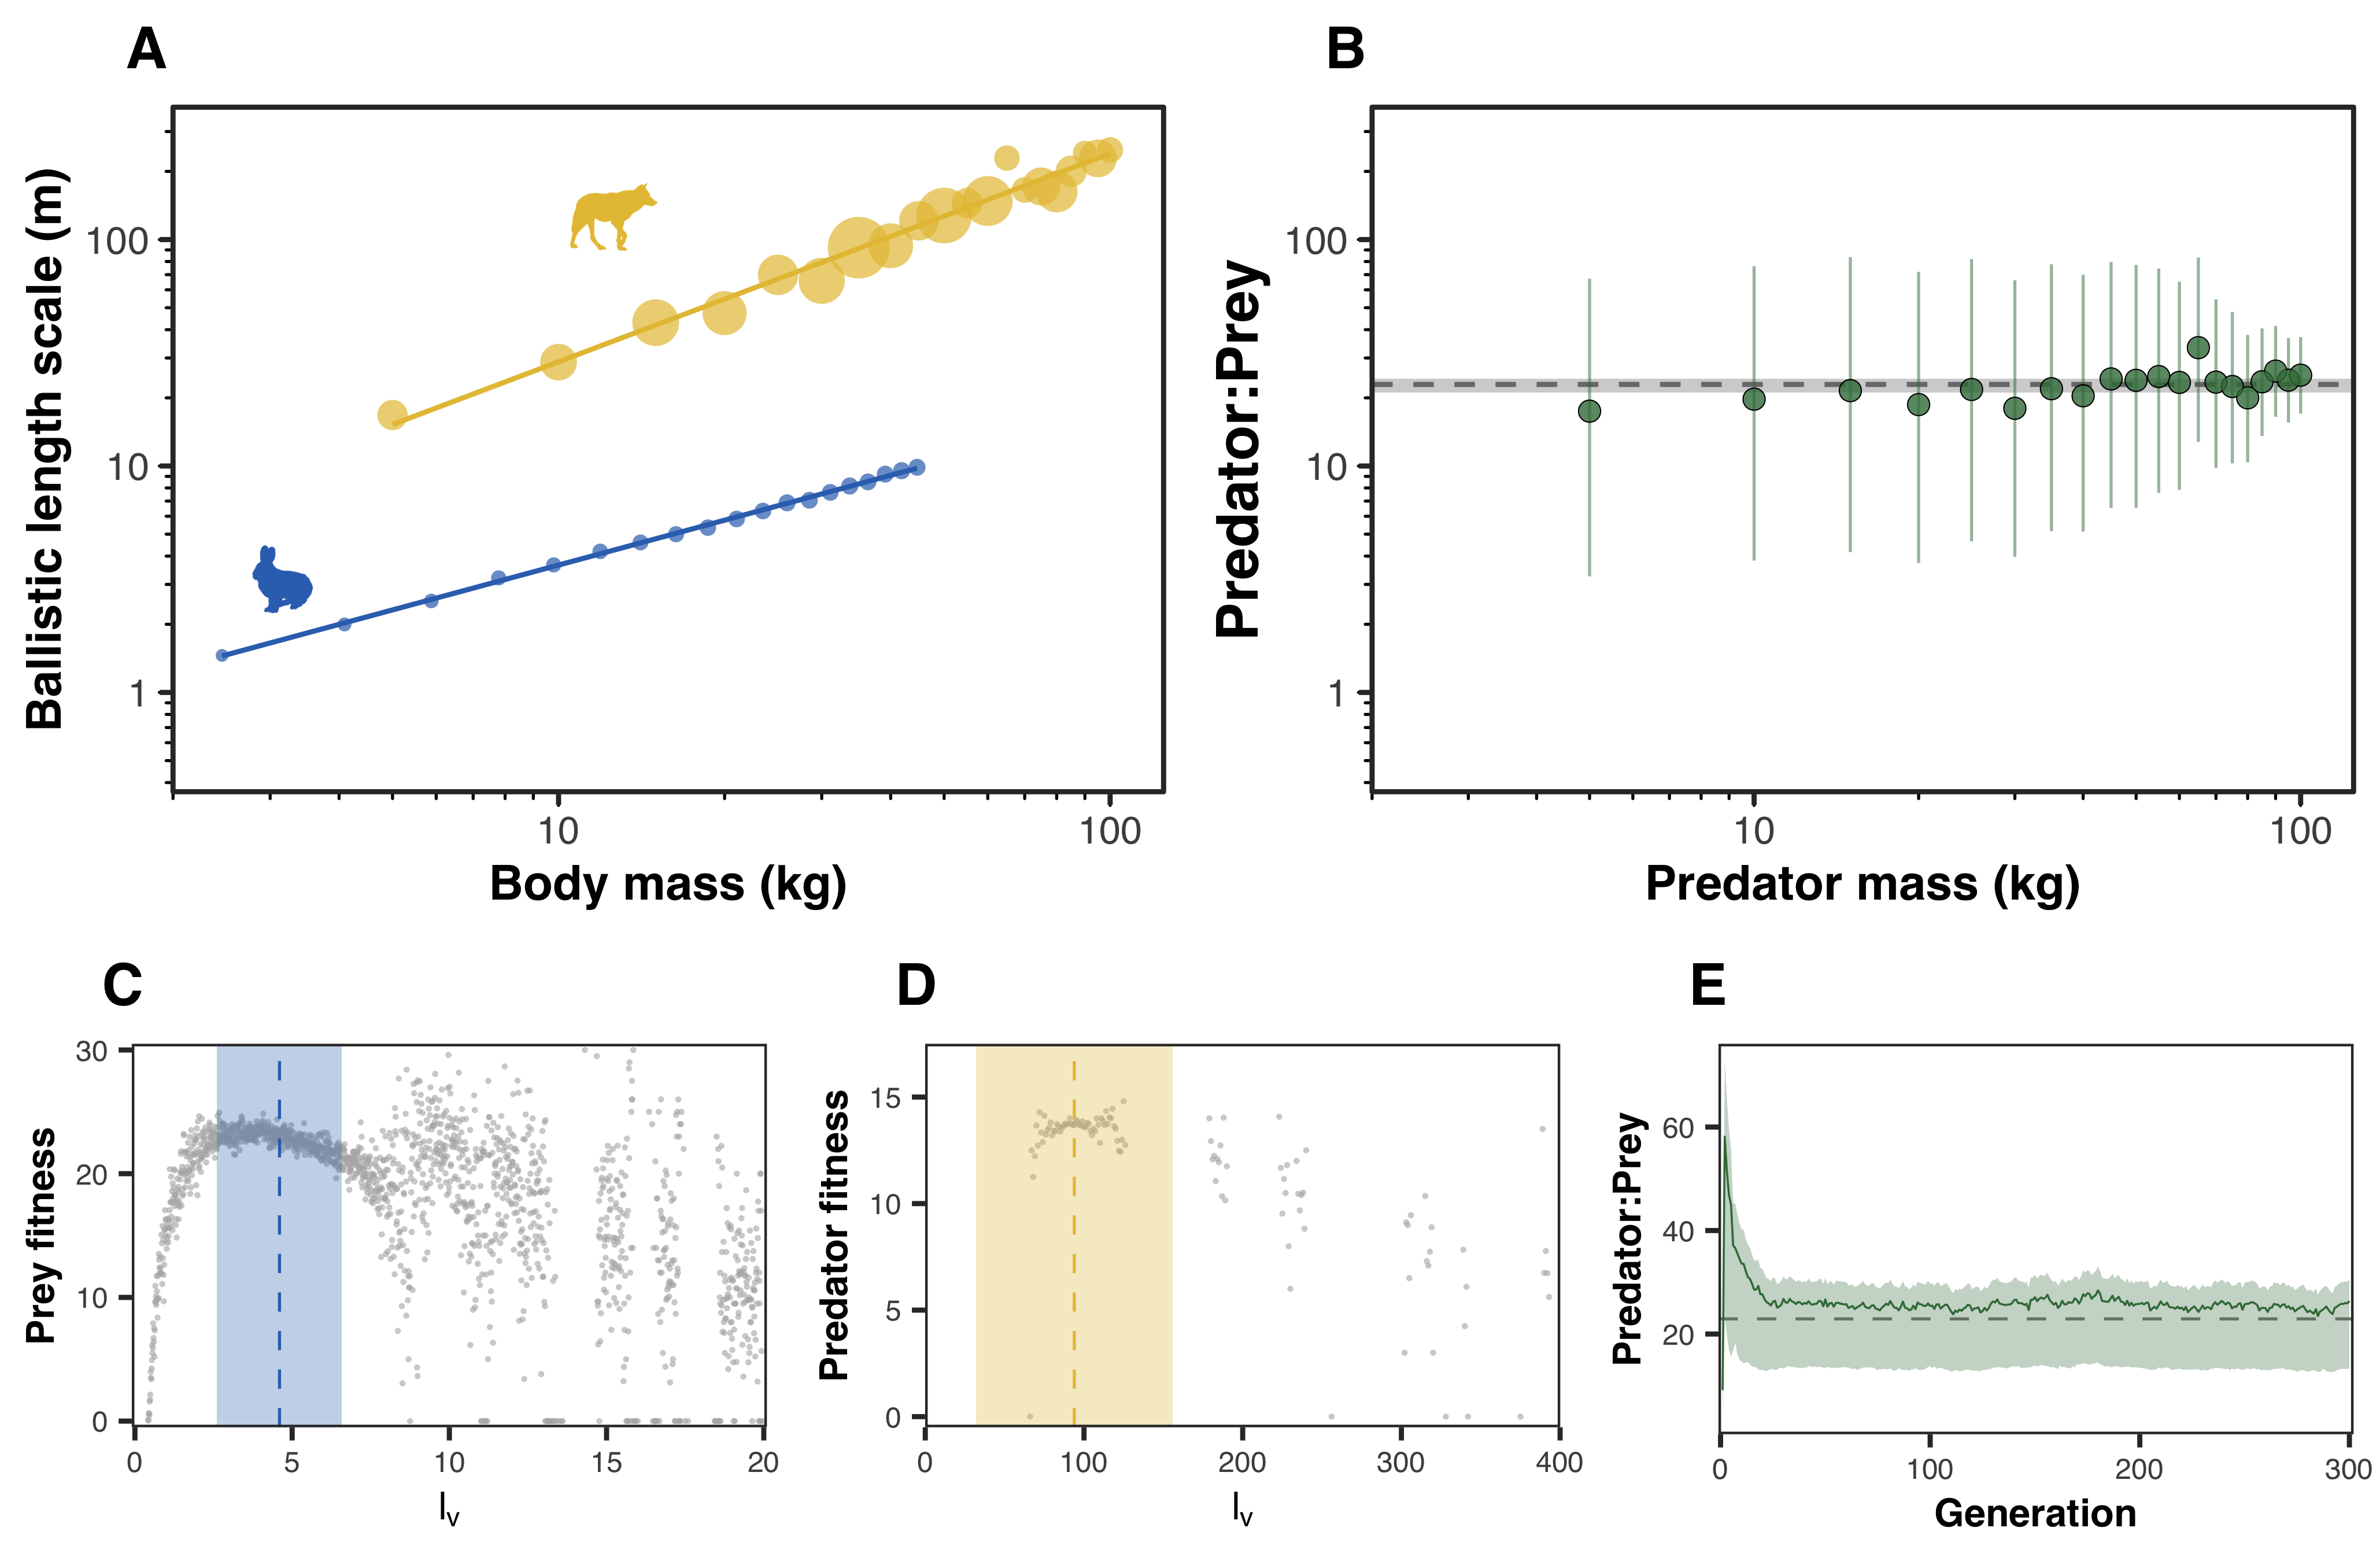
\includegraphics[scale=0.9]{lv_Scaling_Simulations.png}
\caption{Results of our simulation study exploring the evolution of ballistic length scales, $l_v$ in predator-prey systems. Panel A shows the allometric relationship in $l_v$ for both predator (yellow) and prey (blue) species. Panel B shows how the resulting ratio of predator:prey ballistic length scales is mass invariant. The lower three panels depict the fitness C, movement paths D, and pairwise dynamics E for an a single predator-prey system with a predator of 40kg and a prey of ca. 14kg. Point sizes in A are proportional to the variance on the estimates.}
\label{fig:sim_res}
\end{figure}


We tested these predictions using GPS location data on 595 individuals from 53 species of terrestrial mammals (Fig.~\ref{fig:emp_res}A). We annotated the individual datasets with mean adult body size (ranging from 0.5 to 4,000 kg), dietary guild (i.e., herbivorous/frugivorous {\it n = }, and carnivorous/omnivorous {\it n = }), median prey mass for those species that consume mammalian prey, and the median mass of all known predators for each species. We restricted all of our analyses to range-resident animals, as evidenced by variogram analysis \cite{Fleming:2014jr}, and used continuous-time stochastic processes to estimate $l_v$ (Fig.~\ref{fig:emp_res}B), for each individual. We accounted for phylogenetic inertia by including the matrix of phylogenetic distances among species as a random effect in our regressions models.

We found significant positive correlations between $l_v$ and mass for both herbivorous/frugivorous ($t = 5.05$, $p \textless 0.001$), and carnivorous/omnivorous mammals ($t = 3.49$, $p \textless 0.005$; Fig.~\ref{fig:emp_res}C). Carnivores also tended to exhibit more ballistic movement than comparably sized herbivores, with herbivore $l_v$ scaling with mass as
\begin{equation}
l_v = 0.05M^{0.60},
\end{equation}
versus carnivore $l_v$ scaling as
\begin{equation}
l_v = 0.22M^{0.66}.
\end{equation}


\begin{figure}[!h]
\centering
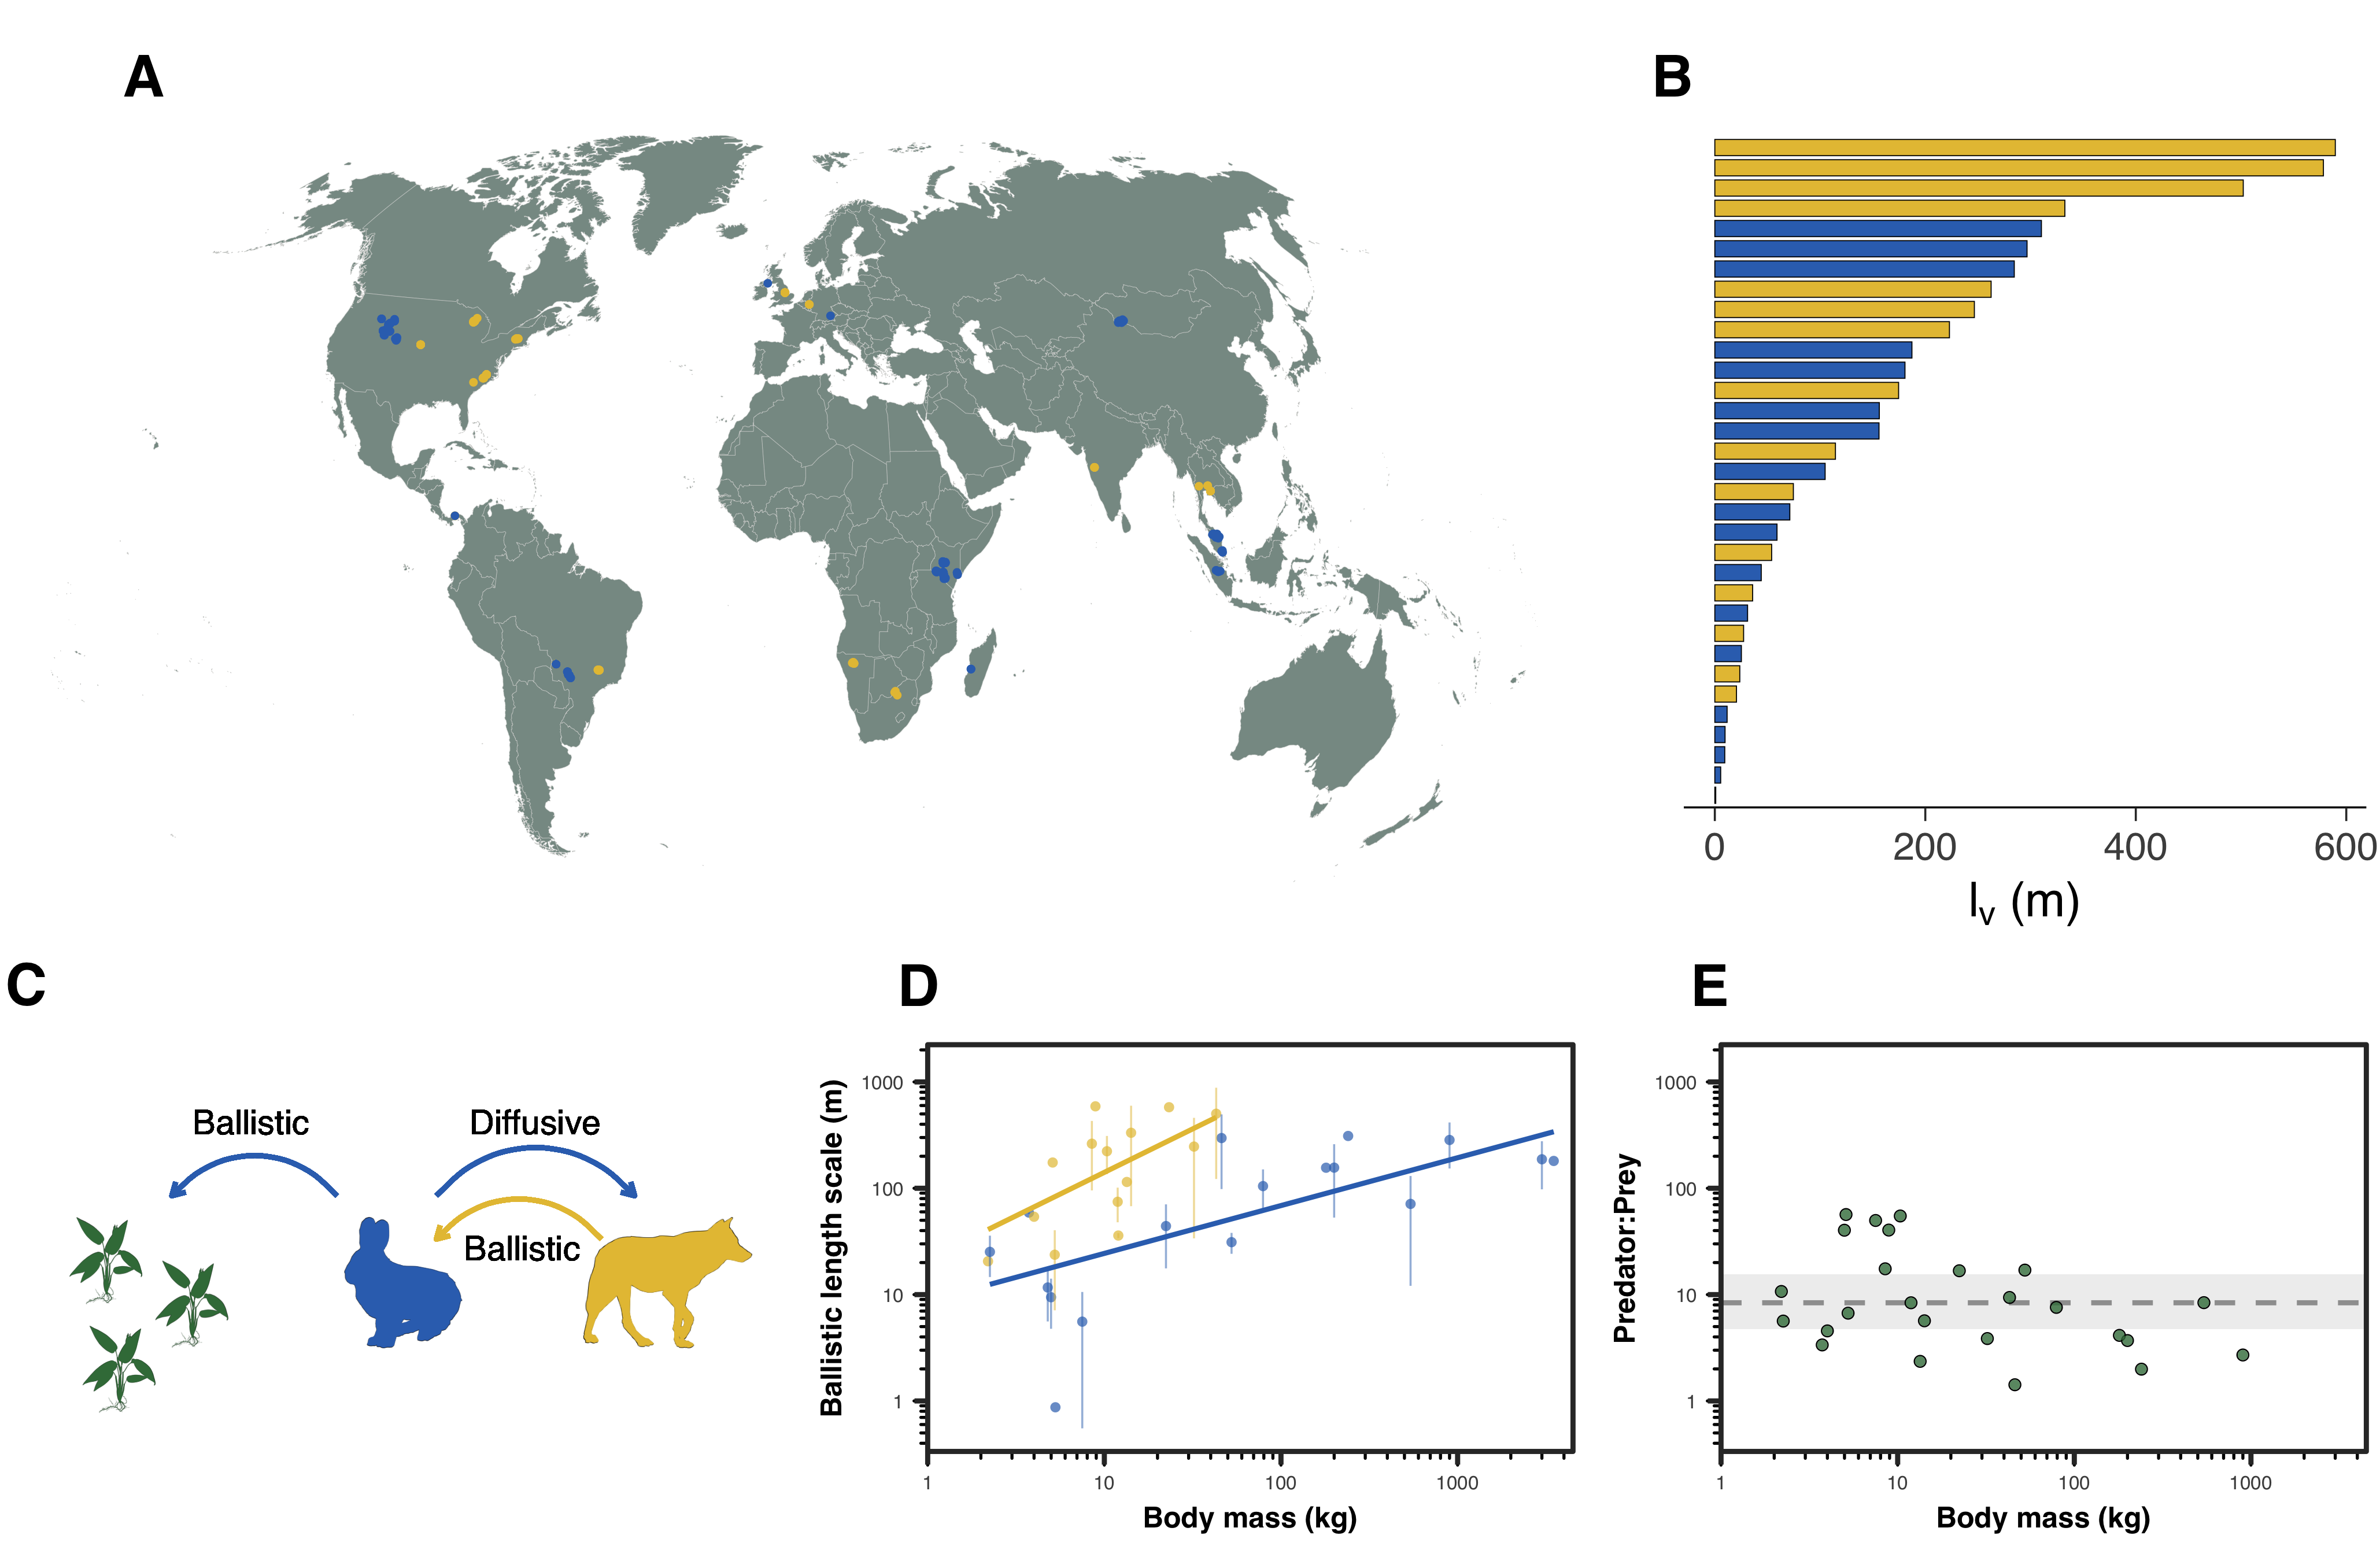
\includegraphics[scale=0.9]{Empirical_Figure.png}
\caption{In A, the GPS relocations of X individuals across YY species plotted on the global map in Winkel Tripel projection; and B shows species median ballistic motion length scales, $l_v$. The lower two scatterplots depict D the allometric scaling of the ballistic length scale, $l_v$ for herbivorous/frugivorous (blue), as well as carnivorous/omnivorous (yellow) mammals; and E the lack of any allometry between the ratio of a predator's $l_v$ to their prey's $l_v$. The axes are log-scaled. The solid lines in D depict the phylogenetically controlled fitted regression models, and the dashed lines in E depict the median ratio.}
\label{fig:emp_res}
\end{figure}


Interestingly, $l_v$ for both feeding guilds scaled with the ca. $\frac{2}{3}$ expected via Euclidean geometry as opposed to the $\frac{3}{4}$ expected under strictly metabolic scaling \cite{Brown:2004}. Although $\l_v$ scaled with mass across 5 orders of magnitude, the best fit models for the ratio between the $l_v$ of predators and their prey (Fig.~\ref{fig:emp_res}D), and between prey and their predators (Fig.~\ref{fig:emp_res}E), were intercept only models. We found that $l_v$ in predatory species tended to be $\sim$18-times longer than their prey. Prey species, in contrast, tended to have an $l_v$ that was $\sim$1/3 of their predators'. 

%When simulating across potential $\tau_v$ ratios, we found that both the mean encounter rate, and mean number of encounters over the duration of the simulation exhibited saturating relationships when increasing a predator's $\tau_v$ for a fixed prey $\tau_v$ (Fig. \ref{fig:sim_res}). When compared to the empirically observed ration of $\sim$3.5, the simulations suggested that increasing $\tau_v$ any further would increase the encounter rate, but with diminishing returns. In contrast, if predator movement was any more diffusive than their prey's movement, their was a non-linear decrease in encounter rates. \todo{Double check numbers in this paragraph}\\


\noindent THINGS TO TOUCH ON IN `DISCUSSION': 

 The $\frac{2}{3}$ scaling expected via Euclidean geometry as opposed to the $\frac{3}{4}$ expected via the metabolic theory of ecology is interesting. Suggests $l_v$ my be primarily a function of spacing patterns rather than energetic requirements.

Although the movement of larger animals tends to be more ballistic than that of smaller animals, predator-prey movement is fixed across the mass spectrum

Encounters can be increased in two ways, increasing speed, or increasing directional persistence. Increasing speed increases the energetic cost of movement, so there is a limit beyond which encounters must be optimized via $\tau_v$. All else being equal though, a change in $\tau_v$ means a change in $\tau_p$, so any behaviour related to $\tau_p$ must be factored in (e.g., territorial maintenance).

Meso-carnivores also have to optimise encountering their prey versus encountering their predators. There is likely strong stabilising pressure on $\tau_v$ for these species.

Prey can't modify their predator's movement to reduce encounters, but they can keep their own contribution down by maintaining more diffusive movement while going about their daily routines.



\bibliography{Refs}

\bibliographystyle{Science}





\section*{Acknowledgments}
Include acknowledgments of funding, any patents pending, where raw data for the paper are deposited, etc.

%Here you should list the contents of your Supplementary Materials -- below is an example. 
%You should include a list of Supplementary figures, Tables, and any references that appear only in the SM. 
%Note that the reference numbering continues from the main text to the SM.
% In the example below, Refs. 4-10 were cited only in the SM.     
\section*{Supplementary materials}
Materials and Methods\\
Supplementary Text\\
Figs. S1 to S3\\
Tables S1 to S4\\
References \textit{(4-10)}


\section*{Materials and Methods}

% ----------------------------------------------------------------
% Analytical work
% ----------------------------------------------------------------

\subsection*{Math}

We analyzed the dependence of the mean first encounter time between and prey and its predator. We modeled both prey and predator movement using Ornstein-Uhlenbeck-Foraging (OUF) processes \cite{Fleming:2014jr,Fleming:2014gd} which feature a finite spatial variance, $\sigma_p$, correlated positions, $\tau_p$, and correlated velocities $\tau_v$. The spatial variances and the positional autocorrelation timescales for each model where parameterized according to allometric relationship (\ref{eq:prey-allo})-(\ref{eq:prey-allo-taup}) and (\ref{eq:predator-allo})-(\ref{eq:predator-allo-taup}) for the prey and the predator respectively. We further parameterized the prey:predator body mass ration using the allometric relationship in (\ref{eq:bodymass-sc}).

To obtain the meand first encounter time we simulated $10^5$ independent realizations of a prey-predator pair of OUF processes. In each OUF realization the initial location and velocity of each individual were sorted from their steady-state probability density functions \cite{Fleming:2014jr,Fleming:2014gd}. We ran the simulations using an Euler algorithm for stochastic differential equations with time step $dt=10^{-3}$ to integrate the pair of coupled SDEs that define the OUF process. We stopped each realization when distance between both trajectories was below an encounter distance $q=0.1$. Because our results do not depend qualitatively on the specific value of $q$ and on the distance between home-range centers, we choose these values to make encounters more frequent and thus reduce computation time. 

Our results show that the mean first encounter time increases monotonically with the positional autocorrelation time scale, $\tau_p$, 




\begin{figure}[!h]
\centering
\includegraphics[width=\textwidth]{pair-mfet.png}
\caption{Mean first encounter time in prey predator pair exhibiting OUF movement. Home-range sizes and the positional autocorrelation timescale were parameterized using the allometric scaling laws in (\ref{eq:prey-allo})-(\ref{eq:prey-allo-taup}) and (\ref{eq:predator-allo})-(\ref{eq:predator-allo-taup}) for the prey and the predator respectively. We used a predator body mass of $10$\,Kg and prey mass was calculated using (\ref{eq:bodymass-sc}). The distance between home-range centers is $2$ (m??? NOT SURE IF THIS IS THE LENGTH SCALE IN THE SCALING LAWS).}
\label{fig:mfet-pairs}
\end{figure}







% ----------------------------------------------------------------
% Simulation Study
% ----------------------------------------------------------------

\subsection*{Simulation Study}

We used a series of stochastic simulations to explore how ballistic length scales, $l_v$, might be expected to evolve in predator prey systems across the body mass spectrum. In these simulations, predator and prey movement were free to evolve via natural selection based on a set of initial conditions and fitness functions. Details on these follow.

% Prey movement
\subsubsection*{Prey movement}

Prey movement were simulated based on Ornstein-Uhlenbeck-Foraging (OUF) processes \cite{Fleming:2014jr,Fleming:2014gd} which feature a finite spatial variance, $\sigma_p$, correlated positions, $\tau_p$, and correlated velocities $\tau_v$. For the prey movement models, all initial parameter values were simulated based on established allometric relationships with prey mass estimated by Noonan et al. \cite{Noonan:2020}. The spatial variances were simulated as

\begin{gather}\label{eq:prey-allo}
\log_{10}(\mathrm{95\%~home~range}) = 0.5078955 + 1.372162 \log_{10}(\mathrm{mass}) \\
%\mathrm{VAR}[\mathrm{position}] = \frac{\mathrm{95\%~home~range}}{-2 \log(0.05)  \pi}
\sigma_p = \frac{\mathrm{95\%~home~range}}{-2 \log(0.05)  \pi},
\end{gather}

the positional autocorrelation timescales as

\begin{gather}\label{eq:prey-allo-taup}
\log_{10}(\E[\tau_\mathrm{position}]) = 1.2994292 + 0.8129125 \log_{10}(\mathrm{mass}).
\end{gather}

For the velocity autocorrelation timescales, we sampled all values between the 0 and $\tau_\mathrm{position}$. This parameterization was selected in order to ensure that the founding population exhibited a sufficiently broad range of initial $l_v$ values on which selection could act. In most real systems, home range size and range crossing times are likely to be highly, and inflexibly, correlated \cite{Noonan:2020}, whereas $\E[\tau_\mathrm{velocity}]$ is likely to be the more flexible parameter. This parameterization thus decreased computation time without compromising biologically realism.

%\begin{gather}
%\log_{10}(\E[\tau_\mathrm{velocity}]) = -1.365200 + 0.787177 \log_{10}(\mathrm{mass}).
%\end{gather}

Variance was then added around the initial values of $\E[\tau_\mathrm{position}]$ and $\E[\tau_\mathrm{velocity}]$ by drawing from chi-square distributions with expectation values of $\E[\tau_\mathrm{position}]$ and $\E[\tau_\mathrm{velocity}]$ respectively. Across all simulations, the home range centers of the prey movement processes were drawn from an isotropic bivariate Poisson distribution.

% Predator movement
\subsubsection*{Predator movement}

Predator movement were also simulated based on OUF processes. For the predator movement models, all initial parameter values were again simulated based on established allometric relationships with prey mass estimated by Noonan et al. \cite{Noonan:2020}. The spatial variances were simulated as

\begin{gather}\label{eq:predator-allo}
\log_{10}(\mathrm{95\%~home~range}) = 1.089972 + 1.478050 \log_{10}(\mathrm{mass}) \\
\sigma_p = \frac{\mathrm{95\%~home~range}}{-2 \log(0.05)  \pi},
\end{gather}

and the positional autocorrelation timescales as

\begin{gather}\label{eq:predator-allo-taup}
\log_{10}(\E[\tau_\mathrm{position}]) = 1.612761 + 0.766461 \log_{10}(\mathrm{mass}).
\end{gather}

For the velocity autocorrelation timescales, we again sampled all values between the 0 and $\tau_\mathrm{position}$

%\begin{gather}
%\log_{10}(\E[\tau_\mathrm{velocity}]) = -0.1005302 + 0.7403169 \log_{10}(\mathrm{mass}).
%\end{gather}

Variance was then added around the initial values of $\E[\tau_\mathrm{position}]$ and $\E[\tau_\mathrm{velocity}]$ by drawing from chi-square distributions with expectation values of $\E[\tau_\mathrm{position}]$ and $\E[\tau_\mathrm{velocity}]$ respectively. Across all simulations, the home range centers of the predator movement processes were fixed at $0,0$.

% Prey fitness
\subsubsection*{Prey fitness and inheritance}

Simulated prey moved across a grid of homogeneously distributed foraging patches (Fig. \ref{fig:Prey_Example}). Each patch had a fixed energetic value that was calculated based on prey body size as $E_{\mathrm{patch}} = \frac{10^{0.774 + 0.727\log_{10}(\mathrm{mass})}}{150}$. Although the energetic value of each patch was arbitrarily defined, it acted only as a scaling constant on the number of offspring (details follow) and thus had no influence on any of the results. A sensitivity analysis on patch width revealed a saturating relationship on the ballistic length scale that prey stabilized around. The width of the foraging patches was therefore defined based on prey body mass as $\frac{\sqrt(\sigma_p)}{10}$. This allowed us to minimized the influence of patch size from our simulations. 

\begin{figure}[!h]
\centering
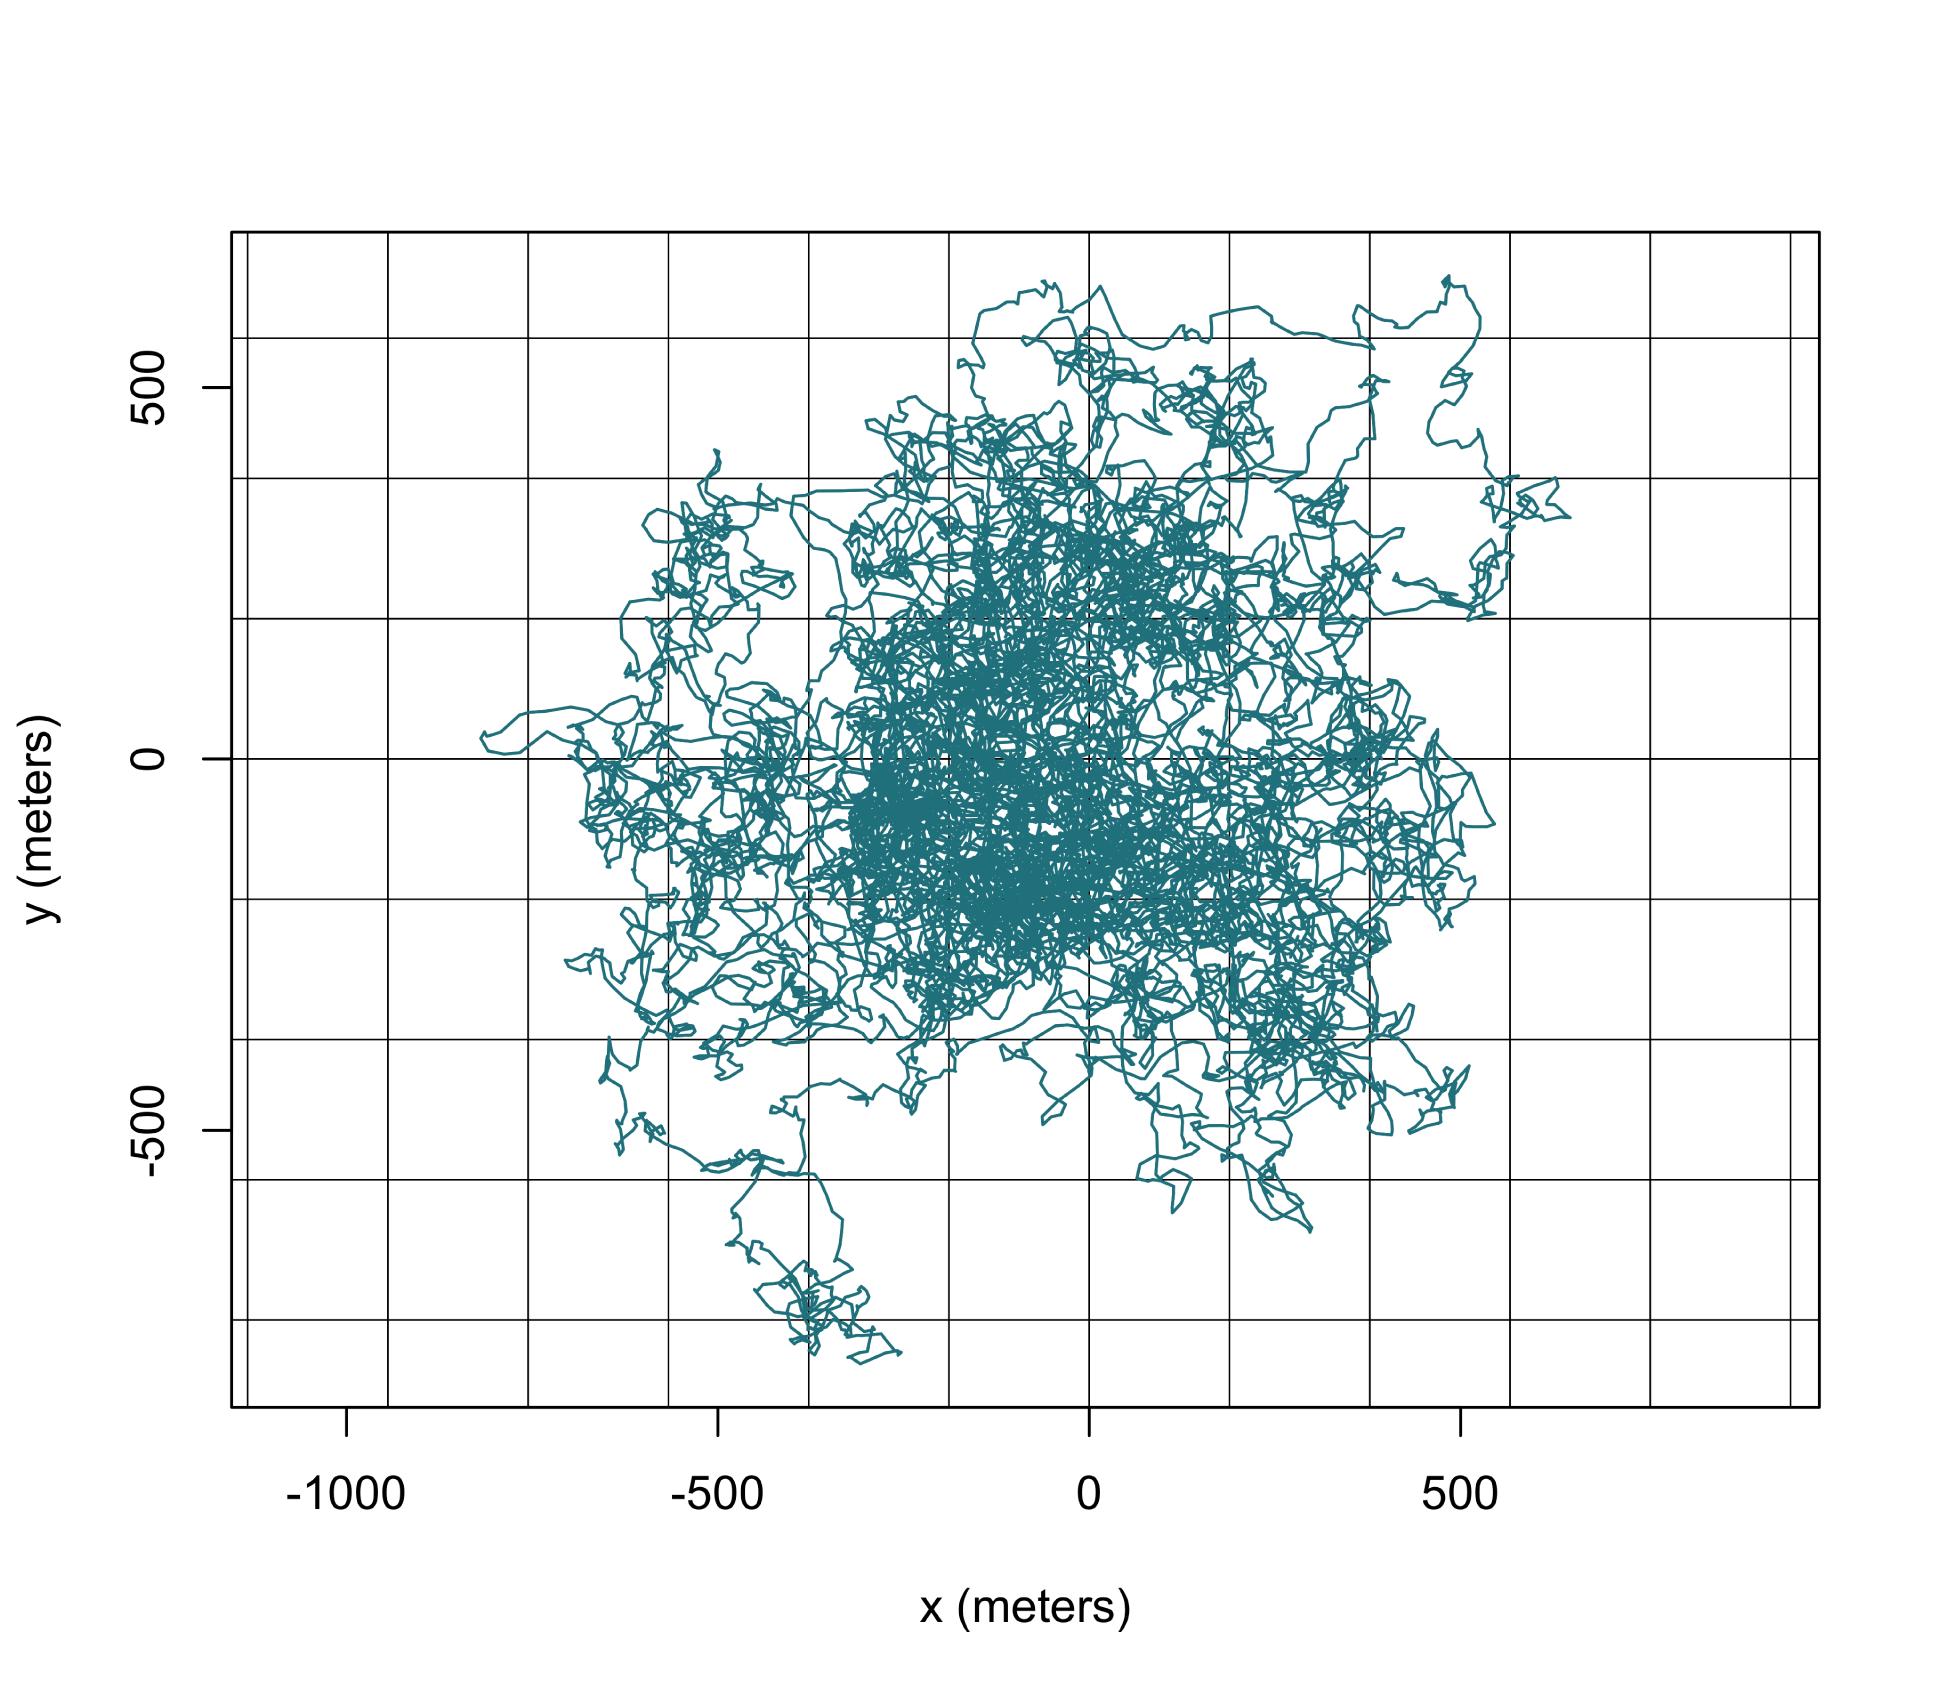
\includegraphics[scale=1]{Prey_Movement.png}
\caption{Example of simulated movement across a grid of homogeneously distributed foraging patches for a $\sim$14 kg prey species. Each patch had an energetic value of 280 kilojoules.}
\label{fig:Prey_Example}
\end{figure}

As prey moved across their foraging landscape, every time they entered a new patch they obtained the full energetic value of that patch. We assumed an instantaneous renewal rate such that every time a patch was (re)entered new energy was available for acquisition. From this, we then defined a prey fitness function based on body mass, total number of kilojoules obtained, movement speed, and predator encounters. Field metabolic rate, FMR, in kj/day was calculated based on the allometric relationships derived in \cite{Nagy:1987} as 

\begin{gather}
\log_{10}(\mathrm{FMR}) = 0.774 + 0.727 \log_{10}(\mathrm{mass}).
\end{gather}

The metabolic cost of movement, $E$, in watts/kg was calculated based on the relationships derived in from \cite{Taylor:1982} as

\begin{gather}
E_{\mathrm{movement}} = 10.7 \mathrm{mass}^{-0.316} \mathrm{speed} + 6.03 \mathrm{mass}^{-0.303}.
\end{gather}
After converting $E$ in watts/kg to kJ/sec, the total energetic cost of movement during the simulation was calculated as:

\begin{gather}
E_{\mathrm{total}} = \mathrm{FMR (\frac{kj}{day}) \cdot duration (days)} + E_{\mathrm{movement}} \mathrm{(\frac{kJ}{sec}) \cdot duration (sec)}
\end{gather}

Because each patch was assumed to have a fixed energetic value, energetic balance at the end of the simulated individual's lifespan was calculated as:
\begin{gather}
E_{\mathrm{Balance}} = E_{\mathrm{patch}} \mathrm{(\frac{kj}{patch})} \cdot \mathrm{number~of~patches} - E_{\mathrm{total}}
\end{gather}

The relationships between energetic costs, patch encounters, and predator movement strategies are shown in Figure \ref{fig:Prey_Diagnostics}.  We then assumed that each day’s worth of excess energy could be converted into a single offspring, such that an individual's total lifetime fitness was calculated as $\frac{E_{\mathrm{Balance}}}{FMR}$. Fitness was rounded down to the nearest whole number and clamped between 0 and $\infty$. All prey that encountered a predator (see below) had a fitness of 0. An individual's offspring then inherited their movement parameters with a small amount of Gaussian distributed noise to emulate intergenerational mutation.

\begin{figure}[!h]
\centering
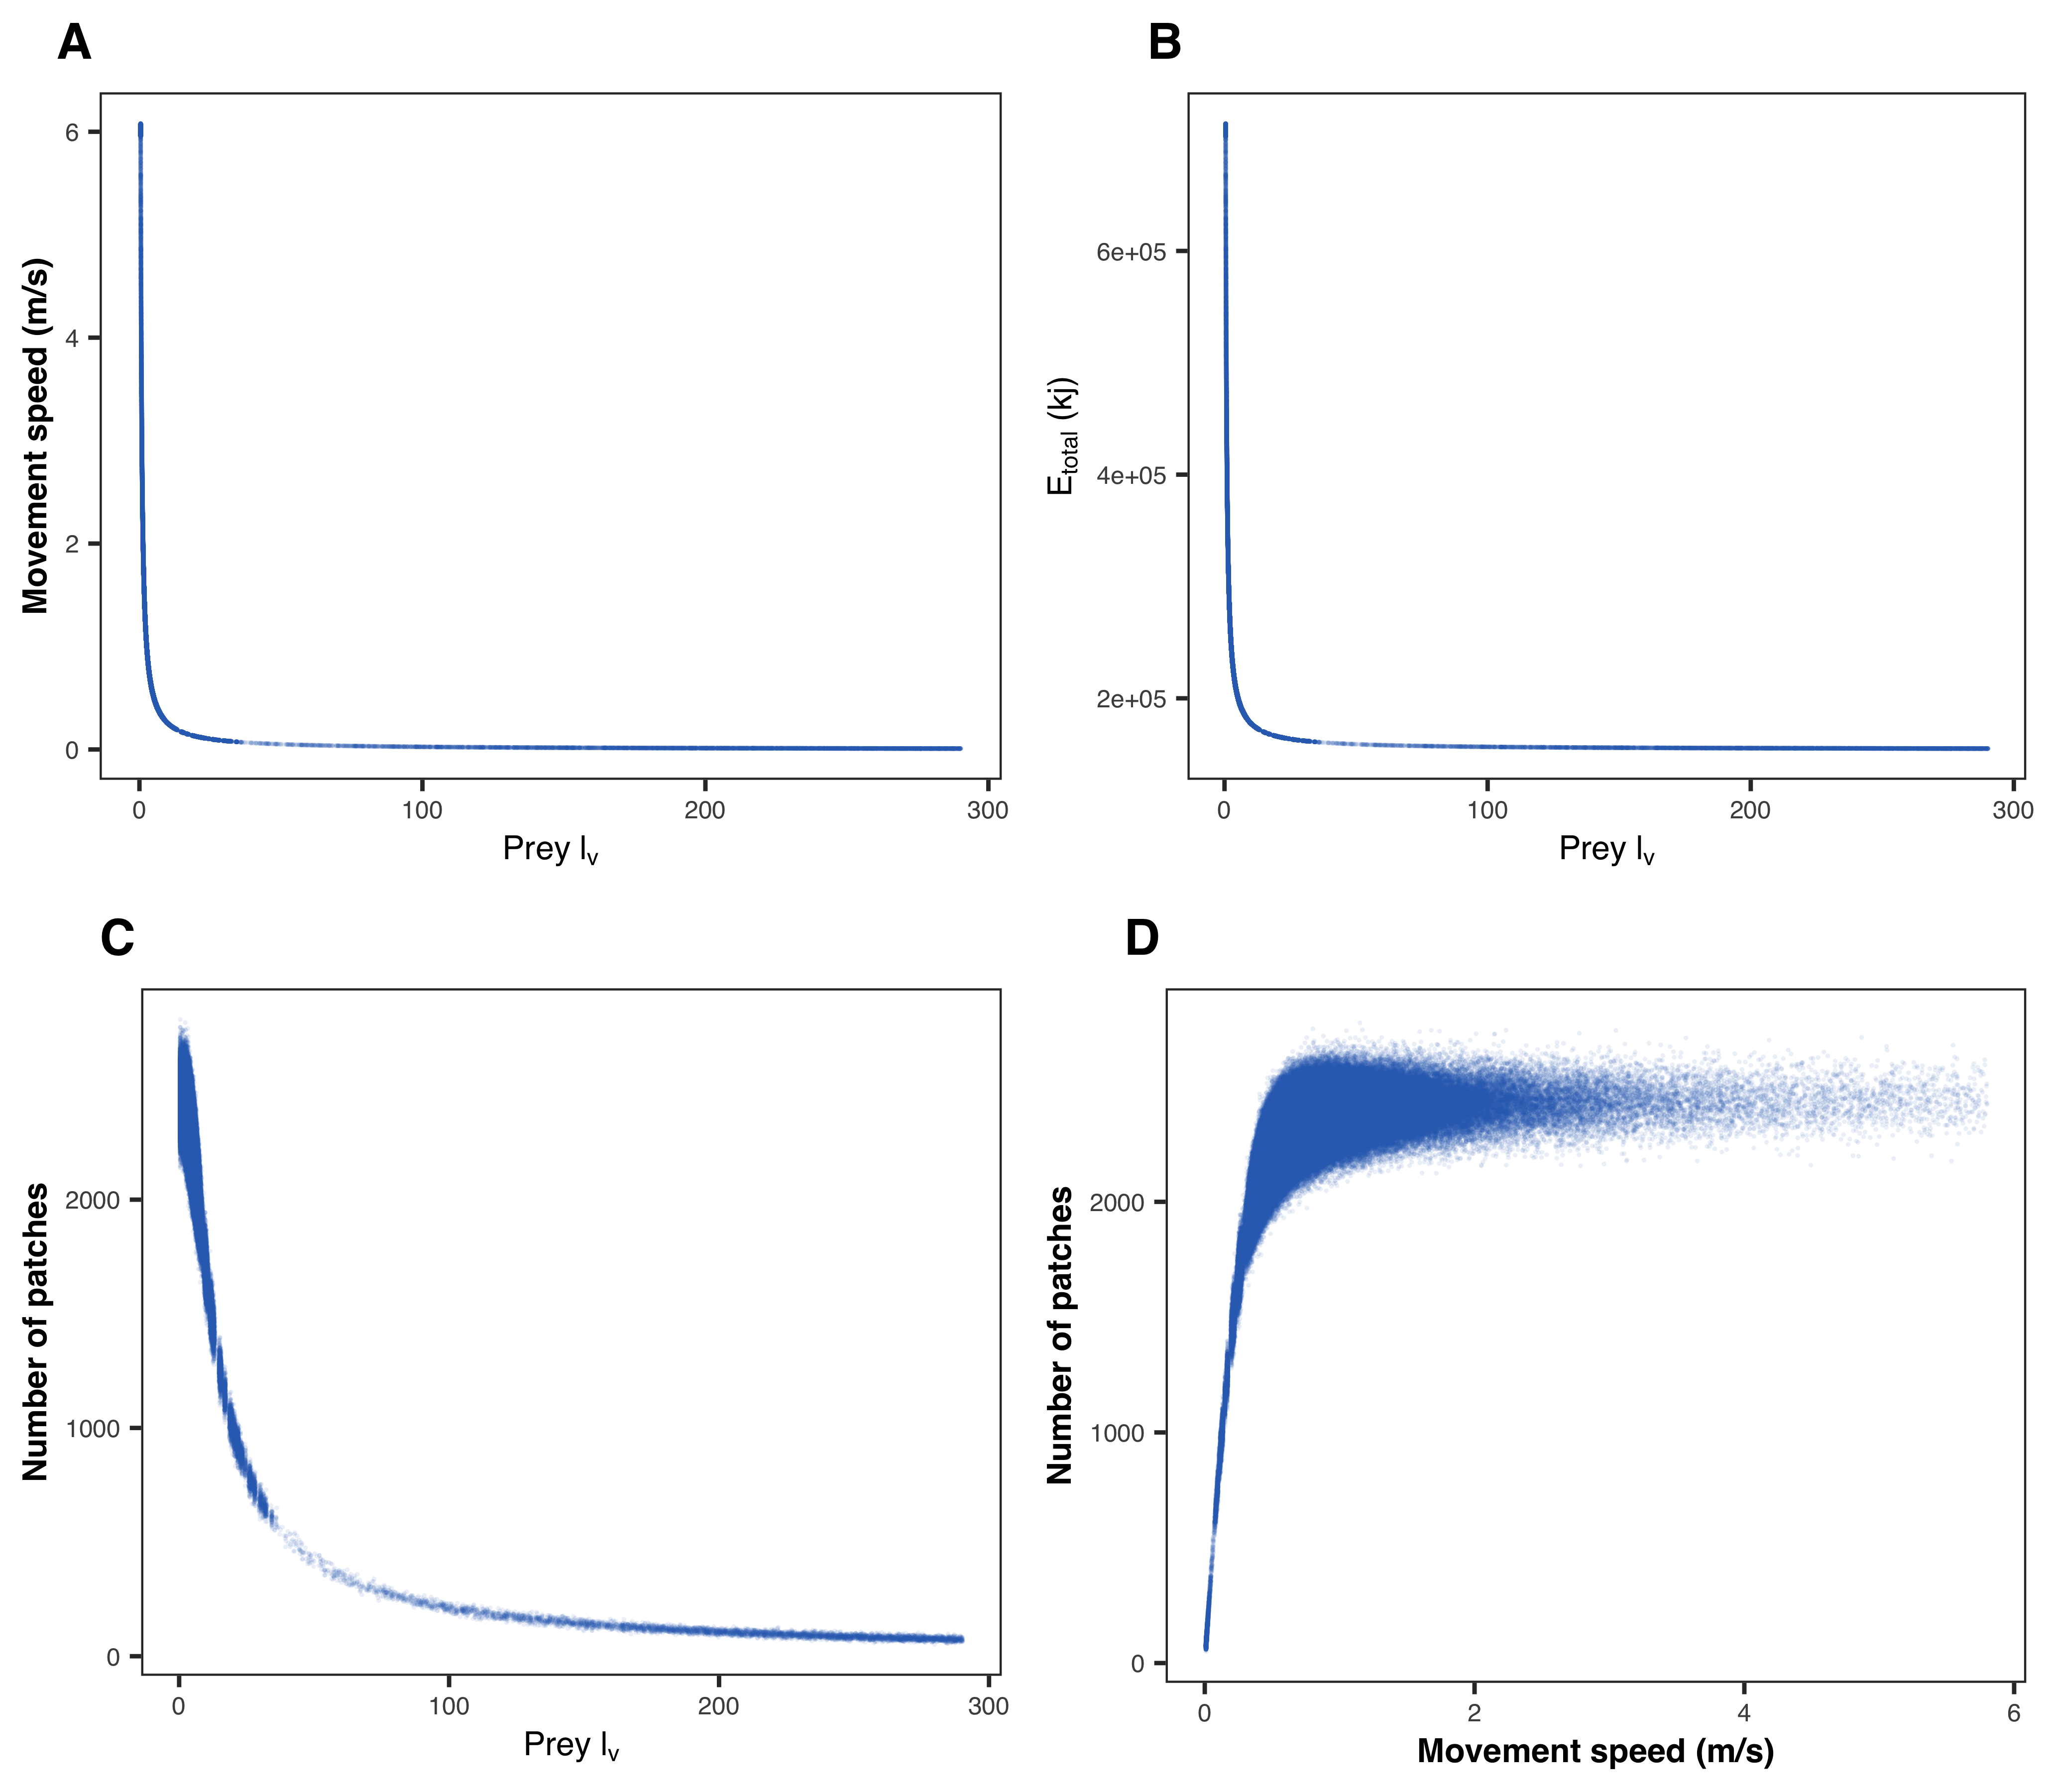
\includegraphics[scale=1]{Prey_Diagnostics.png}
\caption{Scatterplots depicting the relationships between energetic costs, patch encounters, and prey movement strategies for a 14 kg prey species.}
\label{fig:Prey_Diagnostics}
\end{figure}


% Predator fitness
\subsubsection*{Predator fitness and inheritance}

Simulated predators moved across a landscape of randomly distributed prey items (Fig. \ref{fig:Pred_Example}).

\begin{figure}[!h]
\centering
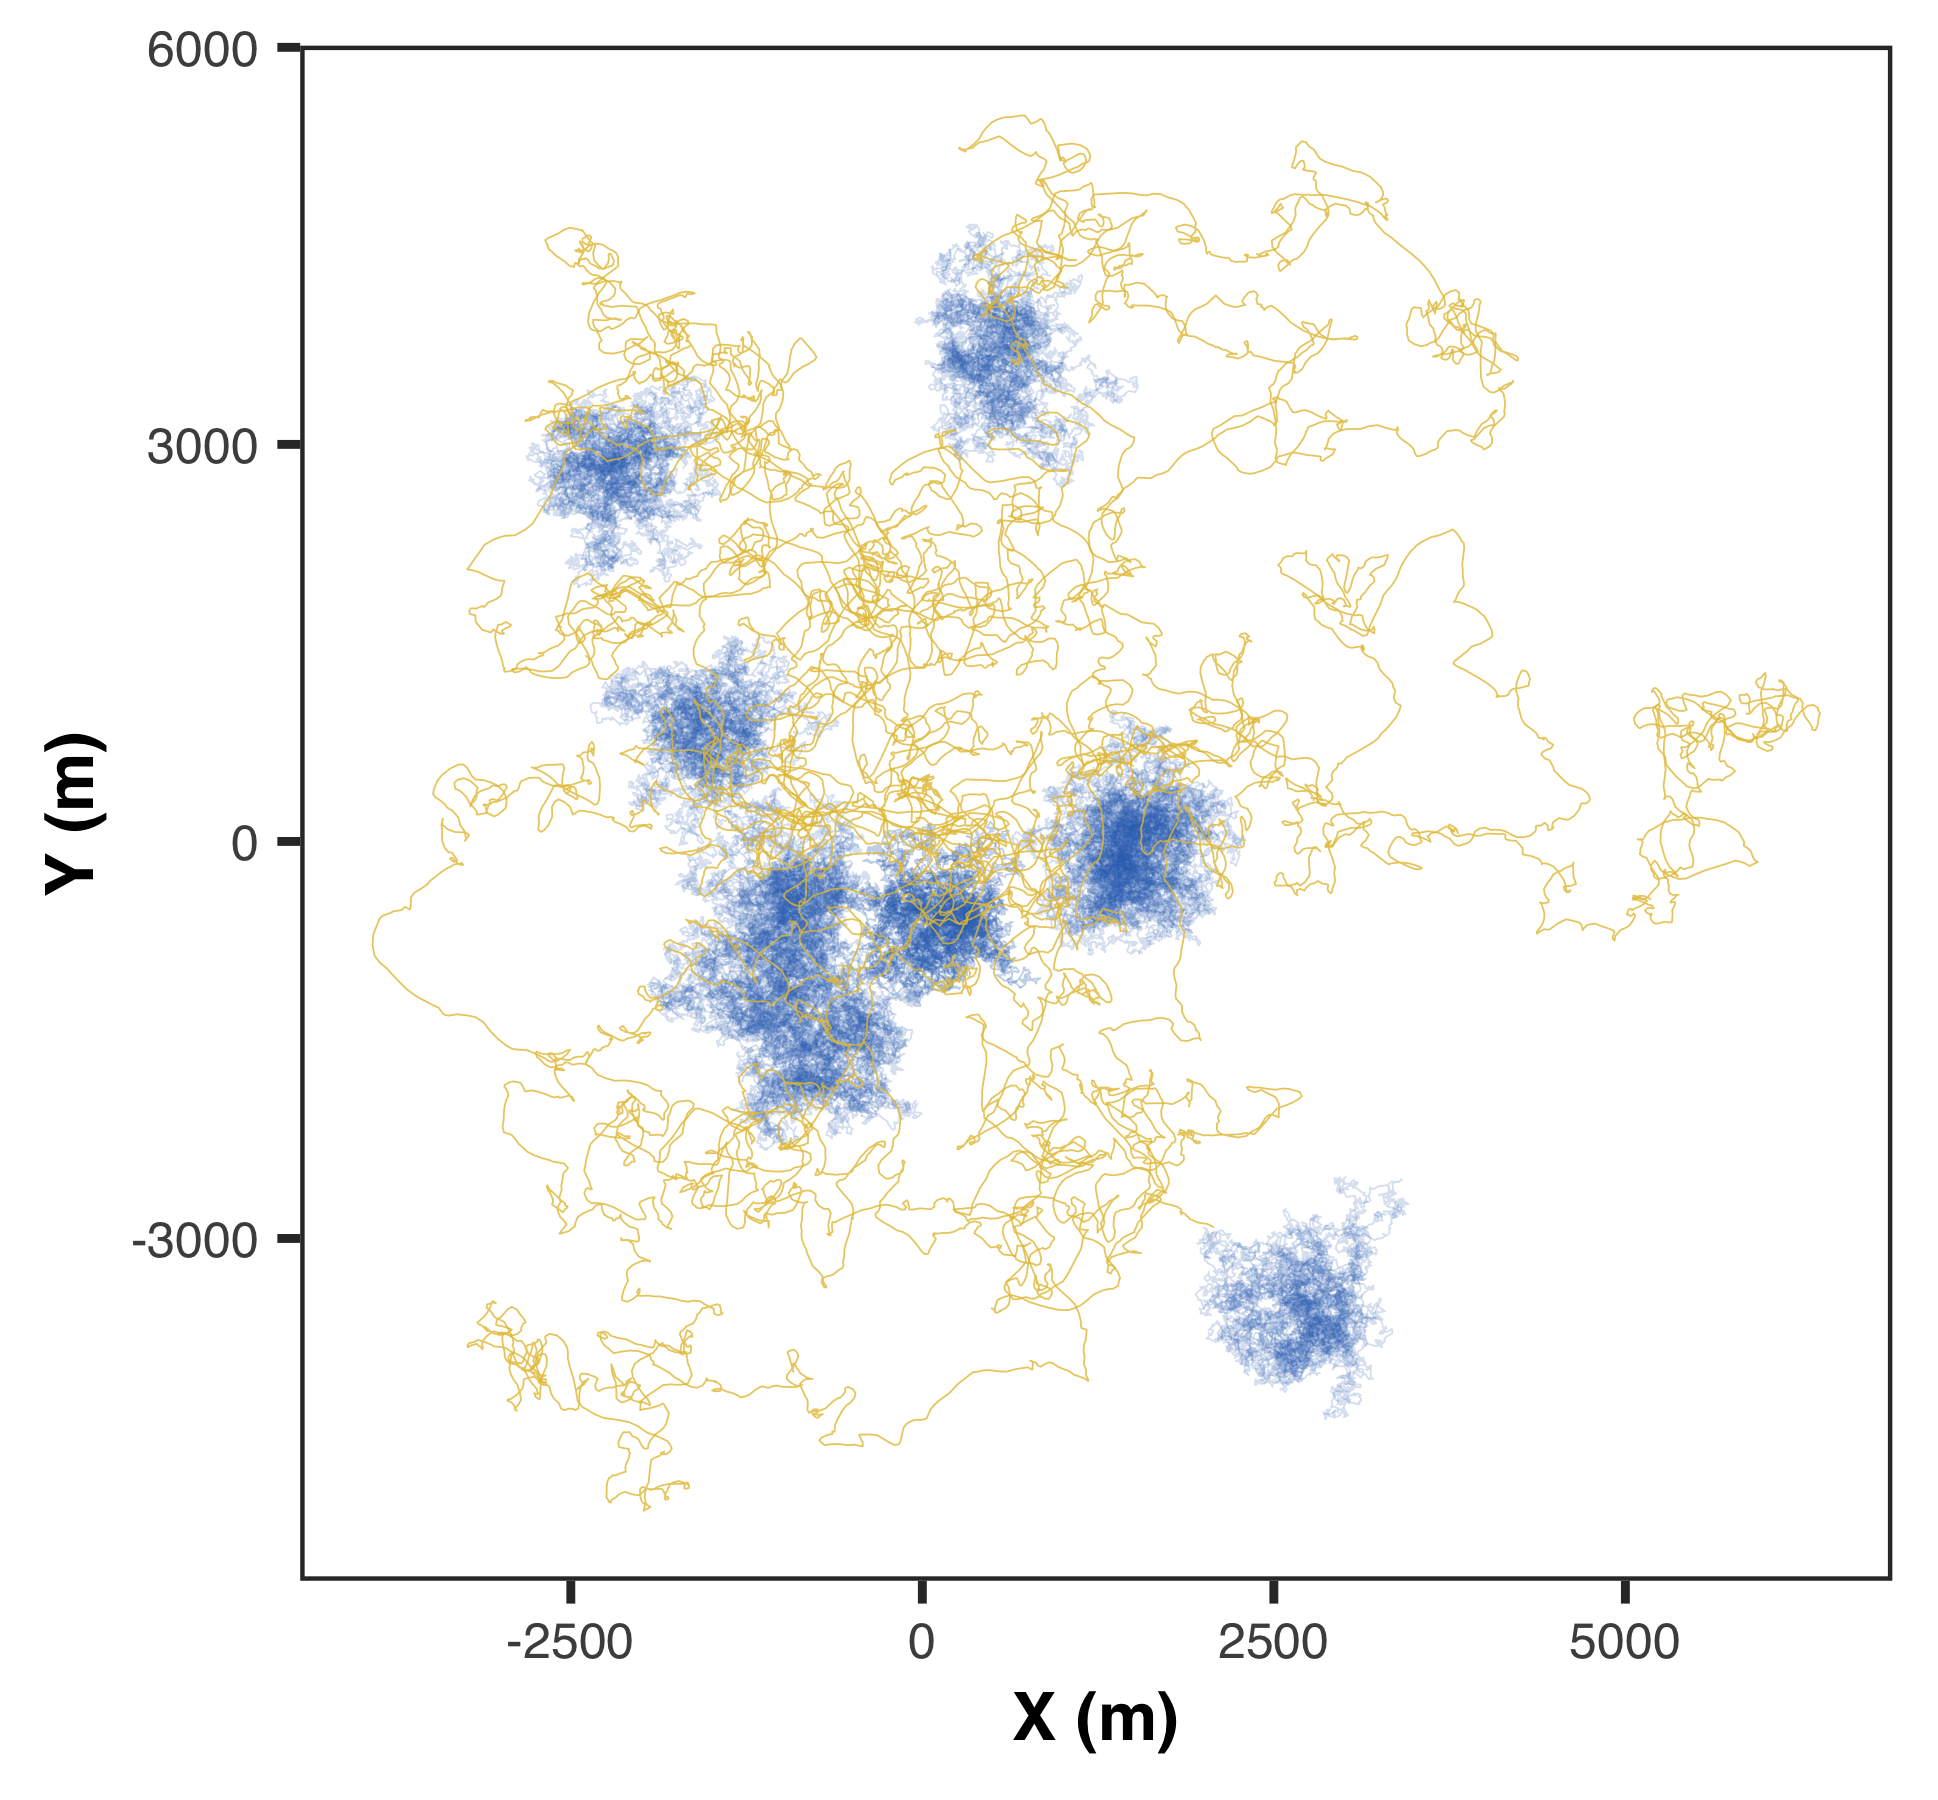
\includegraphics[scale=1]{Sim_Example.png}
\caption{Example of simulated predator movement moved across a landscape of 10 randomly distributed prey items. The predator movement is shown in yellow, whereas the individual prey movement paths are each shown in blue. The home range centers of the prey movement processes were drawn from an isotropic bivariate Poisson distribution, whereas the home range center of the predator movement process was fixed at $0,0$.}
\label{fig:Pred_Example}
\end{figure}

The total energetic cost of metabolism and movement for the predators, $E_{\mathrm{total}}$, was calculated using the same equations as for the simulated prey detailed above. As predators moved across their foraging landscape, every time a prey item entered their perceptual range they were able to capture the prey item and obtain the prey's energetic value. Perceptual range, in m, was defined based on a predator's home range size as $\sqrt(\sigma_p)\cdot 0.05$. Each captured prey item was assumed to have an energetic value of 6.276 kj/g, based on \cite{Gorecki:1965}. Energetic balance at the end of the simulated individual's lifespan was then calculated as:
\begin{gather}
E_{\mathrm{Balance}} = 6.276 \mathrm{(\frac{kj}{g})} \cdot \mathrm{mass_{prey} (g) \cdot number~of~prey}  - E_{\mathrm{total}}
\end{gather}

The relationships between energetic costs, prey encounters, and predator movement strategies are shown in Figure \ref{fig:Pred_Diagnostics}. As with prey fitness, we assumed that each day’s worth of excess energy could be converted into a single offspring, such that an individual's total lifetime fitness was calculated as $\frac{E_{\mathrm{Balance}}}{FMR}$. Fitness was rounded down to the nearest whole number and clamped between 0 and $\infty$. A predator's offspring then inherited their movement parameters with a small amount of Gaussian distributed noise to emulate intergenerational mutation.

\begin{figure}[!h]
\centering
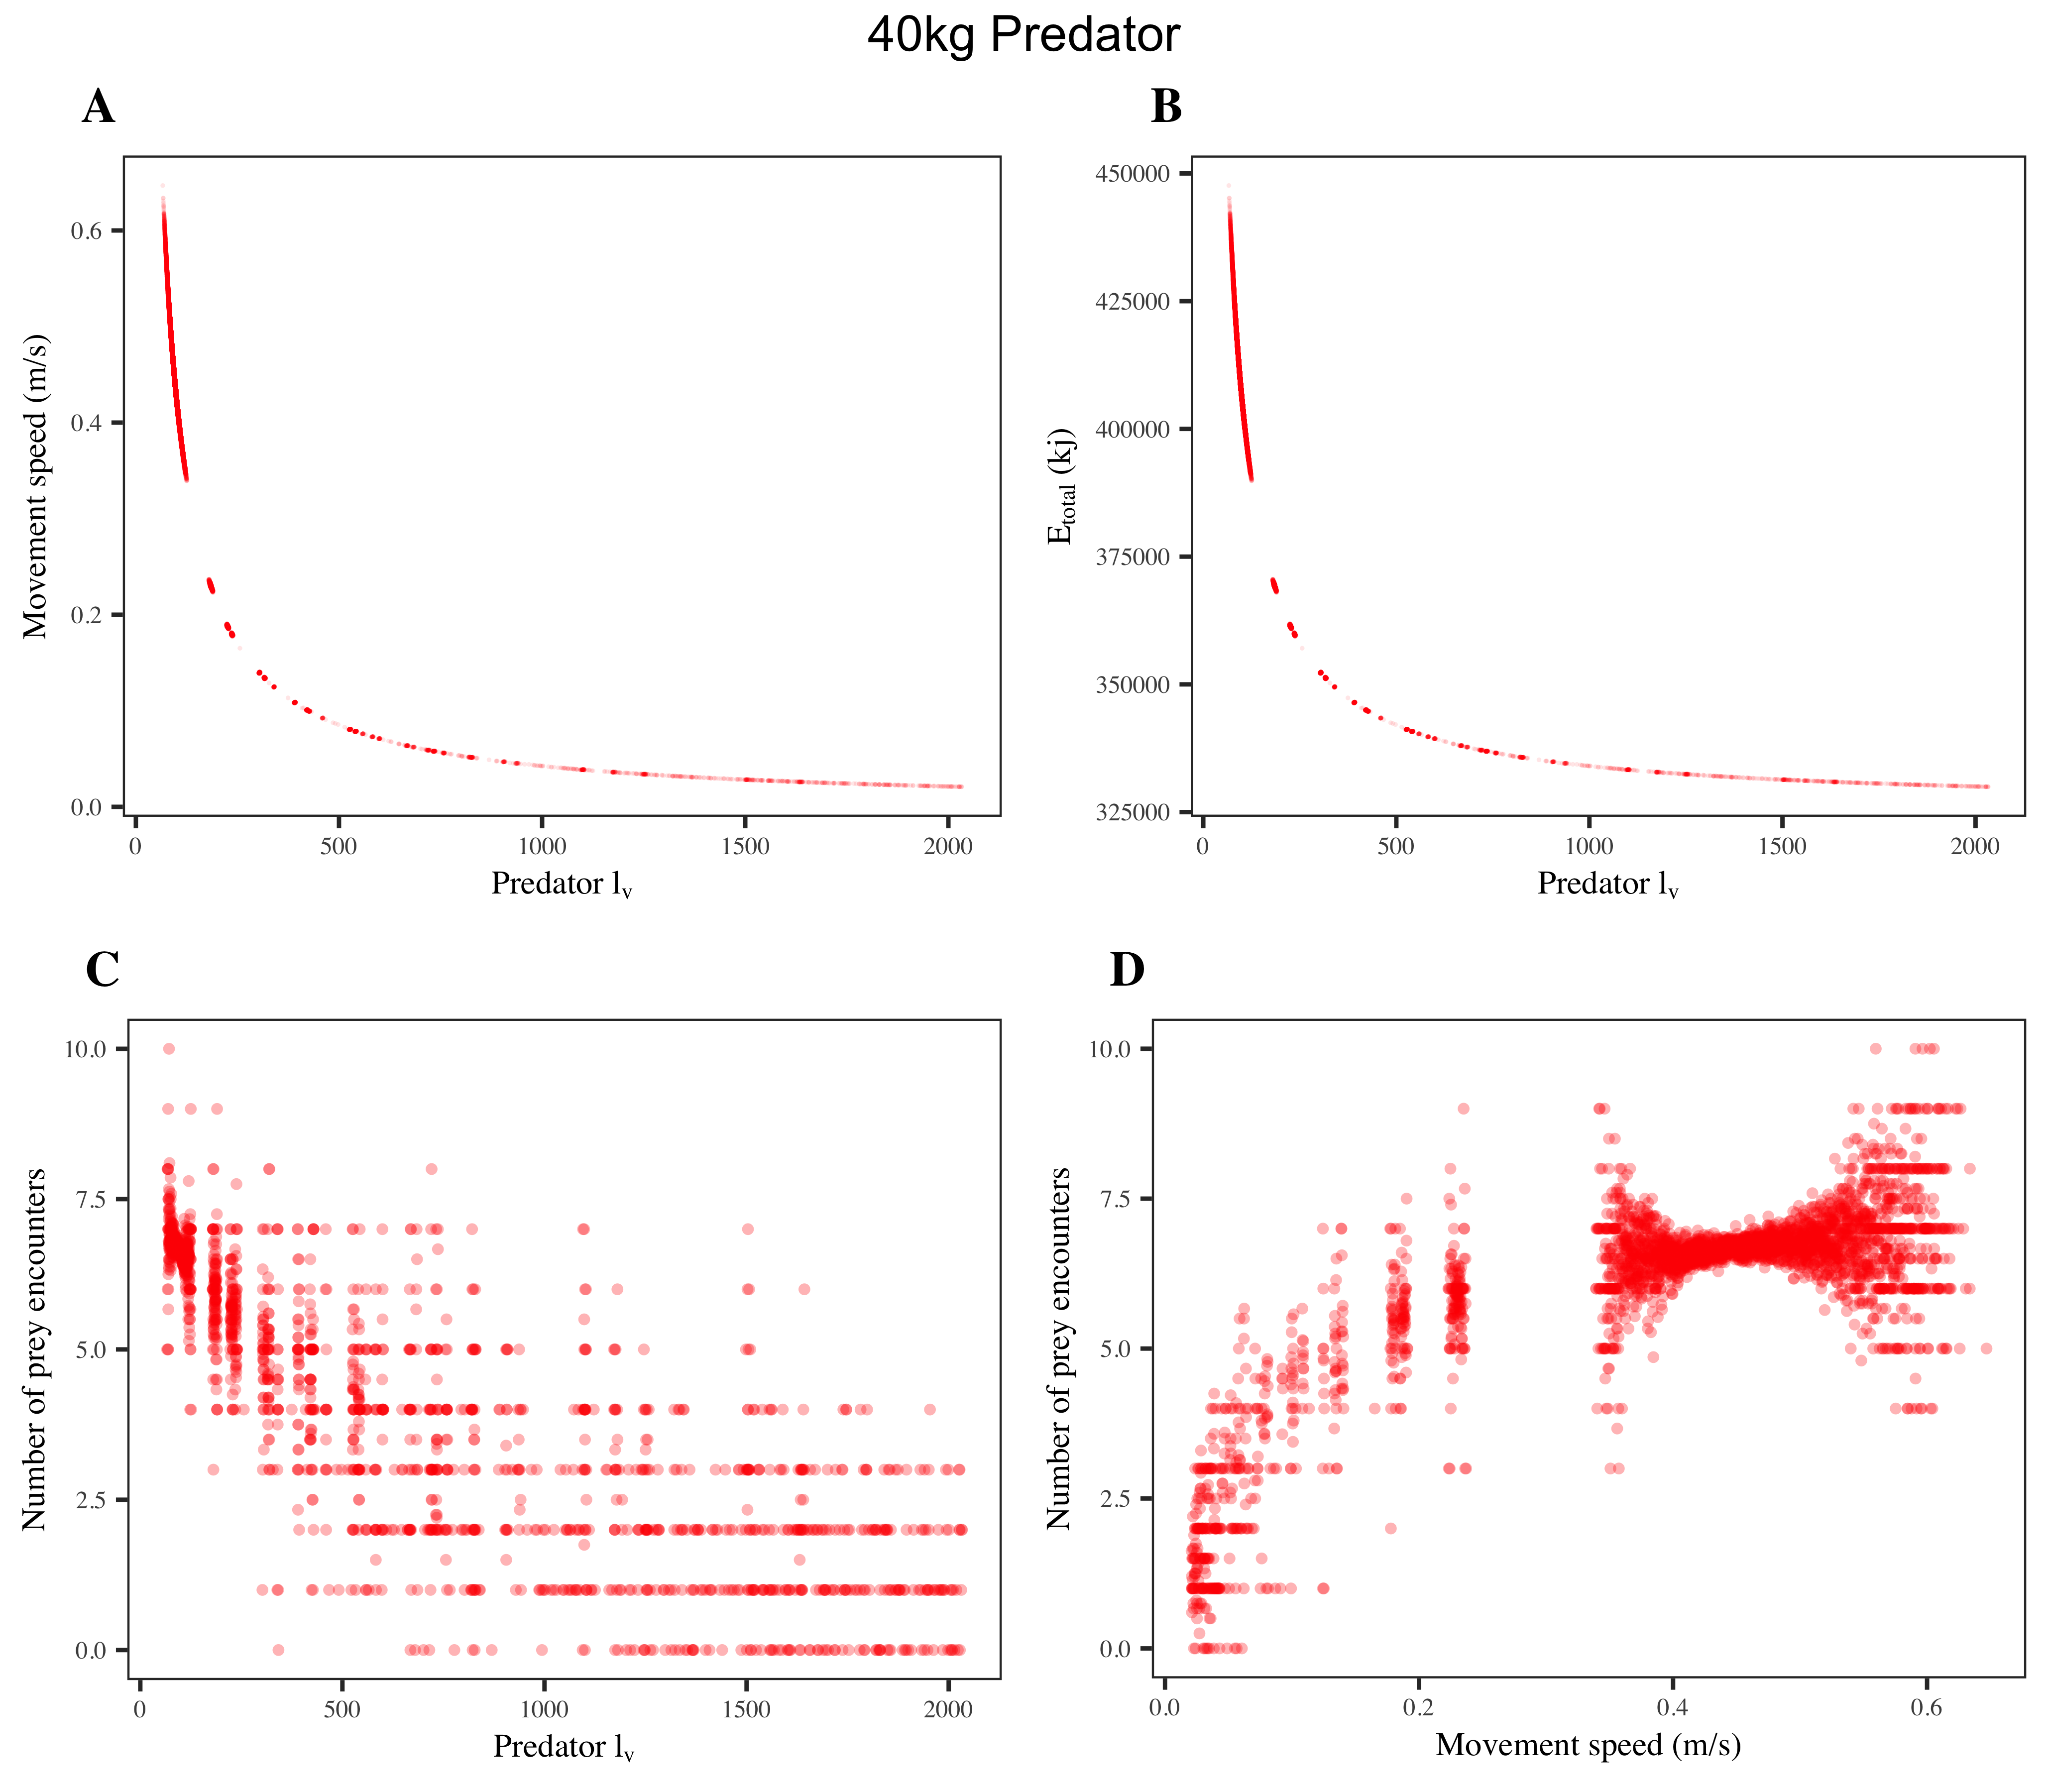
\includegraphics[scale=1]{Predator_Diagnostics.png}
\caption{Scatterplots depicting the relationships between energetic costs, prey encounters, and predator movement strategies for a 40 kg predator species. Note how the general relationships are all consistent with those for the simulated prey shown in figure \ref{fig:Prey_Diagnostics}, but with more stochasticity due to the fact that prey were optimising encounters with stationary foraging patches, whereas predators were optimising encounters with stochastically moving prey.}
\label{fig:Pred_Diagnostics}
\end{figure}



% Simulation setup
\subsubsection*{Simulations}

Our primary aim with this simulation study was to explore how predator-prey dynamics might be expected to evolve across the body mass spectrum. We therefore explored 20 predator-prey systems of various pairwise body sizes. For these we generated 20 pairs of predator and prey founding populations. Predator body sizes ranged between 5 and 100kg by intervals of 5kg, whereas prey body sizes were determined by predator body size using the allometries derived in \cite{Tucker:2014b} 
\begin{gather}\label{eq:bodymass-sc}
\log_{10}(\E[\mathrm{mass_{prey}}]) = -0.87 + 1.26 \log_{10}(\mathrm{mass_{predator}})
\end{gather}
The simulated population consisted of 500 prey and 50 predators with movement parameters for OUF models that were calculated as defined above. Individuals moved within movement `landscapes'. Each landscape consisted of 1 predator, 10 randomly distributed prey, and homogeneously distributed prey foraging patches. This landscape setup was held constant across all simulations in order to avoid and density dependent effects. Individuals moved for a fixed duration of 30 prey range crossings (defined by prey $\tau_p$). Predator and prey fitness were calculated using the functions defined above. Individuals passed on their movement parameters to the following generation based on their fitness. As noted in Eq. (\ref{eq:lv}) the main text, the average length scale over which ballistic motion is maintained ($l_v$, in m) is a function of the spatial variance of an animal's movement process ($\sigma_{\mathrm{position}}$, in m$^2$) and its positional and velocity autocorrelation timescales ($\tau_{\mathrm{position}}$ and $\tau_\mathrm{velocity}$ respectively, in sec). In this regard, we simulated the predator and prey spatial variance $\sigma_{\mathrm{position}}$ based on a purely deterministic model, whereas $\E[\tau_\mathrm{position}]$ and $\E[\tau_\mathrm{velocity}]$ were drawn from chi-square distributions. As such, $\tau_\mathrm{position}$ and $\tau_\mathrm{velocity}$ were the only two parameters defining $l_v$ that were free to evolve by natural selection in our simulations.

At the end of the generation, the landscapes were `refreshed' with new movement models sampled from the available pool of offspring and both fitness and inheritance were calculated anew. This process was then repeated for 300 generations. This resulted in a total of 150,000 selection events for the simulated prey, and 15,000 selection events for the predators. In all cases the predator and prey movement converged to a stable value (Fig. \ref{fig:Convergence}). Once the simulations had completed, we calculated $l_v$ values for all predators and prey for the final 50 generations (i.e., 25,000 prey and 2,500 predators). We then estimated the average ratio of predator:prey ballistic length scales. Confidence intervals on the ratio were estimated use the F-distribution via the methods implemented in the \texttt{ctmm R} package.

\begin{figure}[!h]
\centering
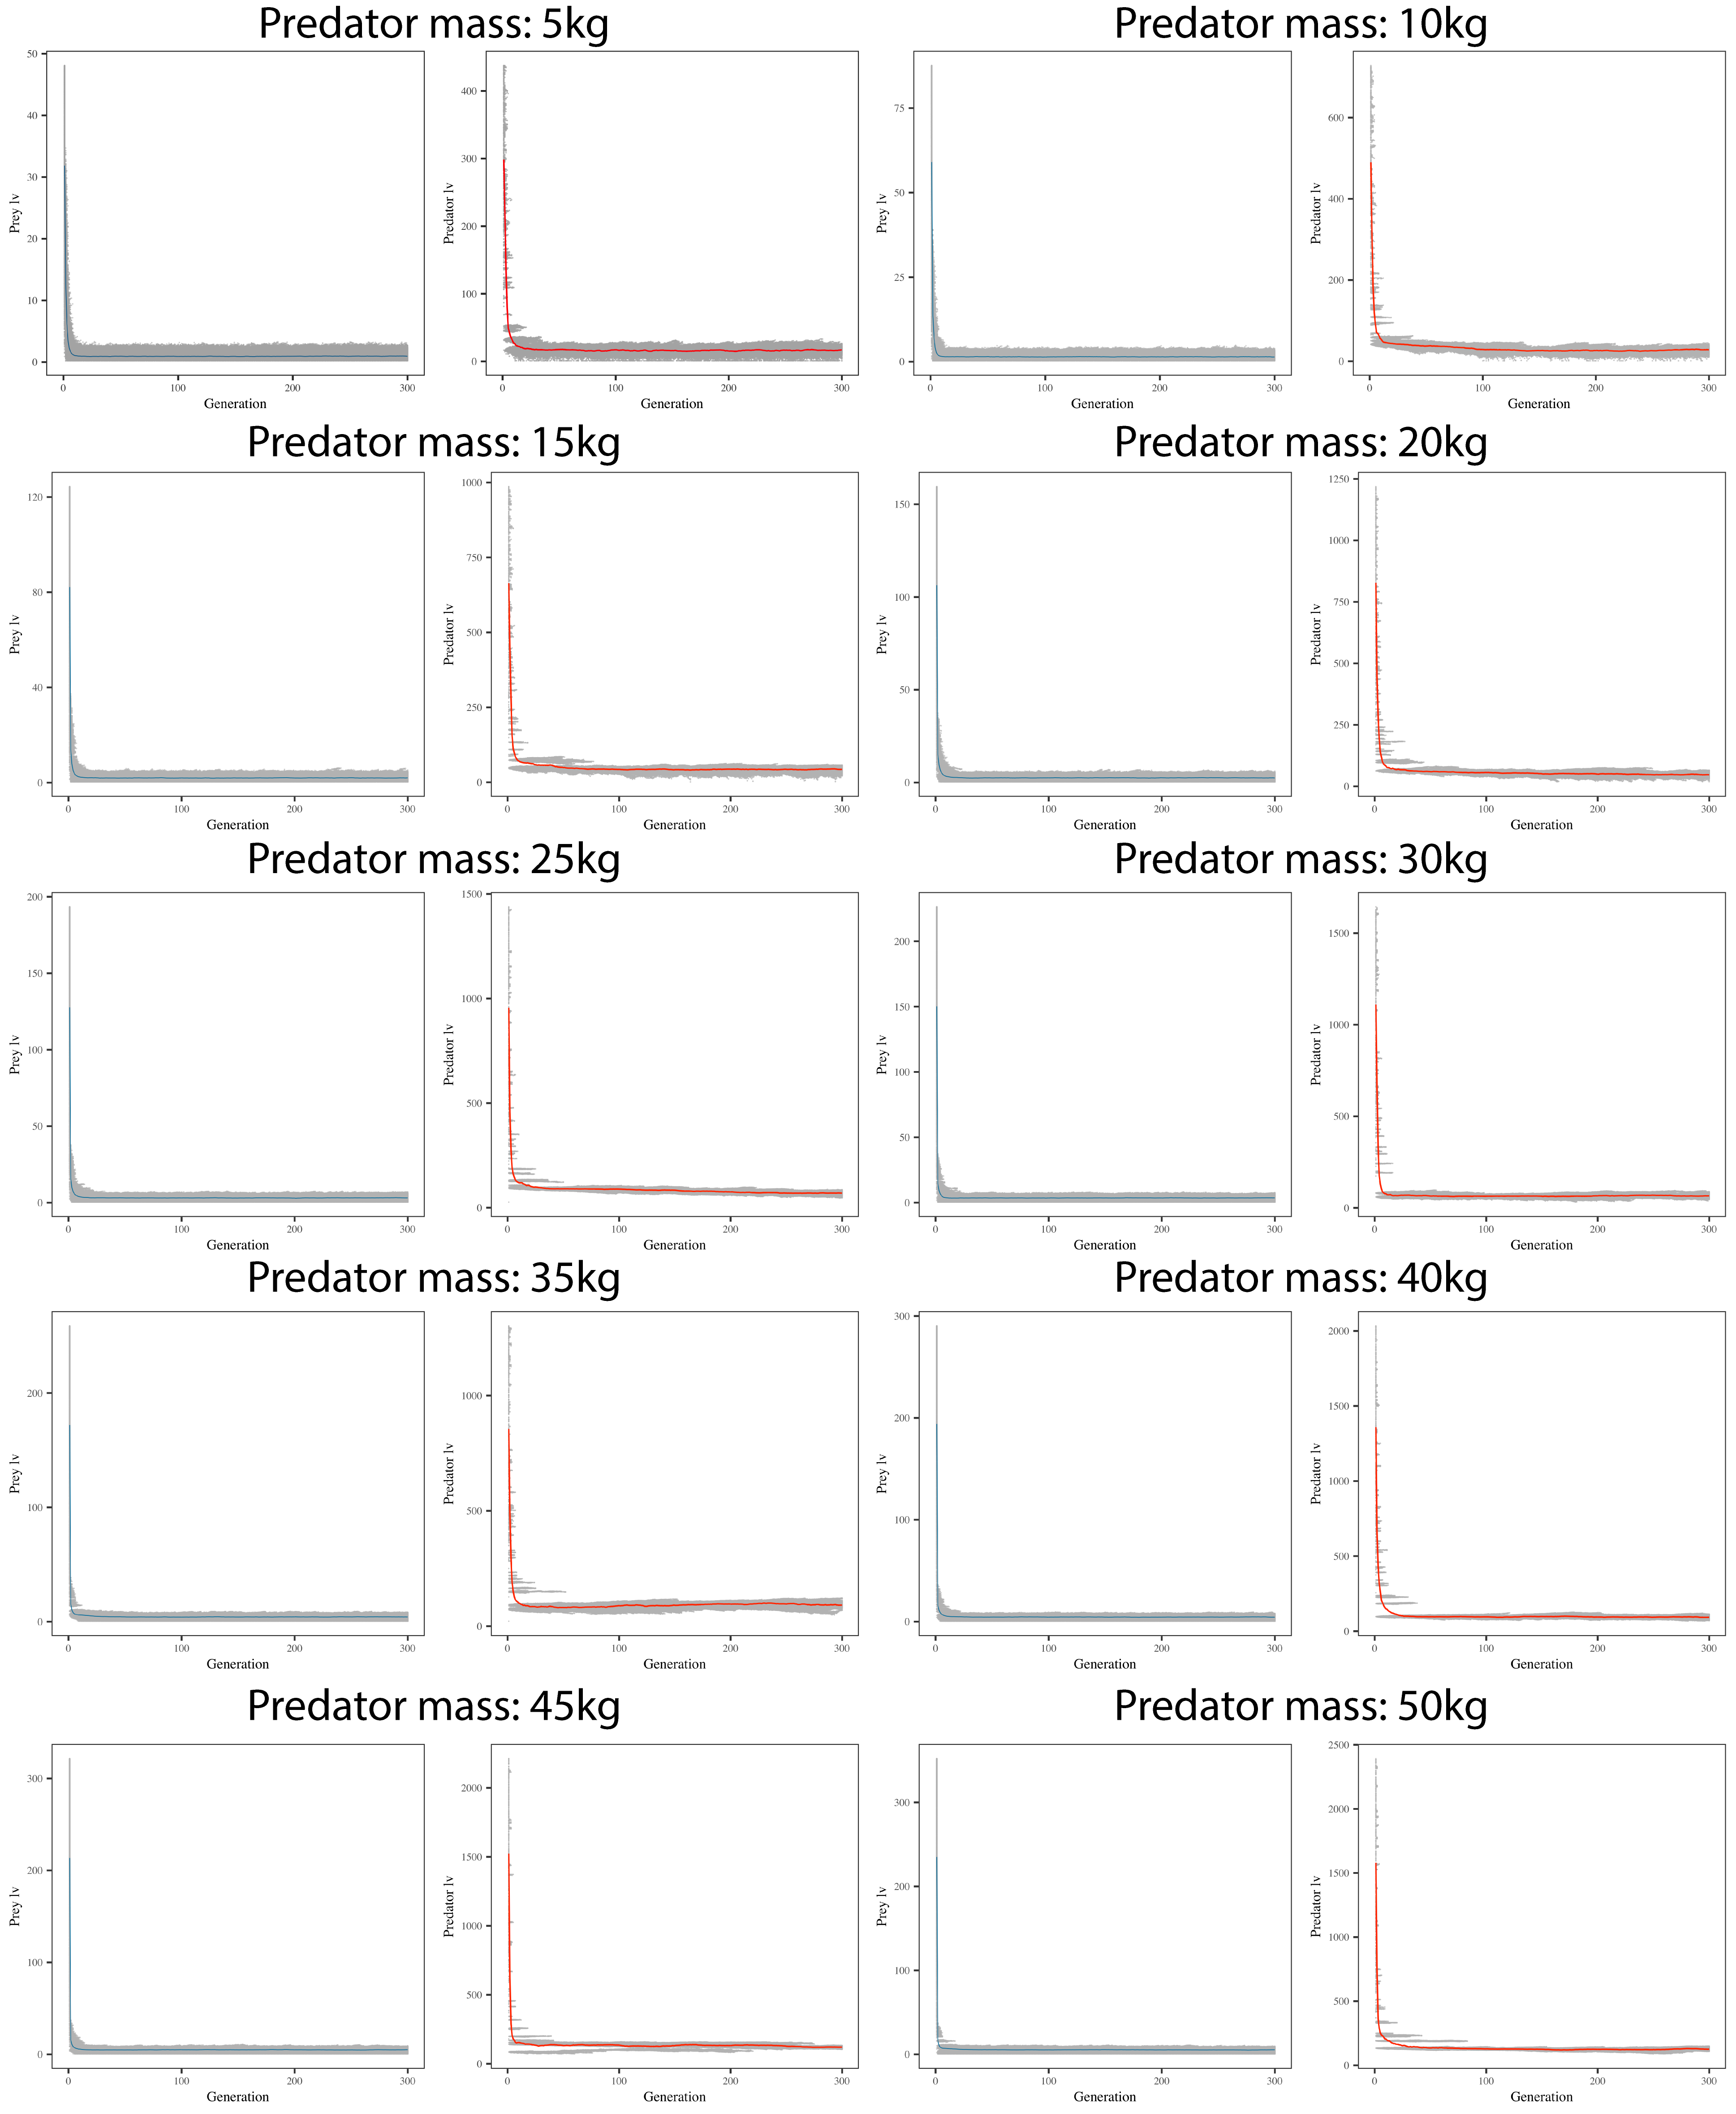
\includegraphics[scale=0.9]{Convergence_Plots.png}
\caption{Scatterplots depicting the ballistic length scales of predators and prey over successive generations. Only the first 10 body size pairs we tested are shown, however, the remaining simulations showed similar patterns of convergences.}
\label{fig:Convergence}
\end{figure}



All of the simulations were carried out using the University of British Columbia's High Performance Computing Cluster (HPCC). All simulations were parallelized to improve performance and the computation time per mass-specific predator prey system was 7 days. With 20 systems explored, this resulted in a total computation time of 140 days. The \texttt{R} scripts used to carry out this simulation study are openly available on GitHub at \url{https://github.com/NoonanM/BallisticMotion}.


% ----------------------------------------------------------------
% Empirical analyses
% ----------------------------------------------------------------

\subsection*{Empirical analyses}

\subsubsection*{Tracking data analysis}

To investigate the potential for ballistic motion to scale allometrically in terrestrial mammals, we compiled GPS tracking data for XXXX species, comprising a total of $XXX$ locations for YYY individuals. Data were obtained from the online animal tracking database Movebank \cite{Wikelski:2017uy}, or contributed by co-authors directly, and are openly available (XXXXXXXX). Notably, this dataset includes species with body masses covering 4 orders of magnitude (0.5 -- 4000 kg), providing the broad coverage of the mass spectrum required to investigate allometric trends. Individual datasets were selected based on the criterion of range resident behavior, as evidenced by plots of the semi-variance in positions as a function of the time lag separating observations (i.e., variograms) with a clear asymptote at large lags \cite{Fleming:2014jr, Calabrese:2016ey}. All data from migratory, or dispersing individuals were excluded as their measured movement strategies would not be representative of the normal foraging dynamics we aimed to quantify. The visual verification of range-residency via variogram analysis \cite{Fleming:2014jr} was conducted using the \texttt{R} package \texttt{ctmm} \cite{Calabrese:2016ey}.

As noted in Eq. (\ref{eq:lv}), the average length scale over which ballistic motion is maintained ($l_v$, in m) is a function of the spatial variance of an animal's movement process ($\sigma_{\mathrm{position}}$, in m$^2$) and its positional and velocity autocorrelation timescales ($\tau_{\mathrm{position}}$ and $\tau_\mathrm{velocity}$ respectively, in sec). Estimating $l_v$ for these data thus first required estimating the autocorrelation structure in each of the individual tracking datasets. To do this, we fit a series of range-resident, continuous-time movement models to the data. The fitted models included the Independent and Identically Distributed IID process, which features uncorrelated positions and velocities; the Ornstein-Uhlenbeck (OU) process, which features correlated positions but uncorrelated velocities \cite{Uhlenbeck:1930fw}; and an OU-Foraging (OUF) process, featuring both correlated positions, and velocities \cite{Fleming:2014jr, Fleming:2014gd}. Model selection was then be employed to identify the best model for the data \cite{Fleming:2014gd, Fleming:2015fo}, from which the positional autocorrelation timescale parameter, $\tau_p$, was extracted. Notably, estimating the autocorrelation structure of the tracking data in this way also provided an estimate of $\hat{N}_\mathrm{area}$. To fit and select the movement models, we used the \texttt{R} package \texttt{ctmm}, applying the workflow described by \cite{Calabrese:2016ey}. Because only the OUF processes included information on all of the parameters required to estimate $l_v$, we further restricted out analyses to only those individuals for which the OUF model was selected. NEED TO INCLUDE STATS ON WHETHER THERE WERE ANY SPECIES/STUDY/GEOGRAPHIC BIASES IN THIS SUBSETTING.

\subsubsection*{Covariate data}

For each of the species in our dataset we compiled covariate data on that species' mean adult mass, in kilograms, take from previously published sources. For the Carnivora, mass data were taken from \cite{Noonan:2015kg}, while data for species from other orders were taken from \cite{Myers:2019}. To investigate the potential influence of diet on movement strategies, we identified the main food source for each of the species in our dataset, defined as constituting at least 60\% of the diet \cite{Gittleman:1985il, Noonan:2015kg}, and classified the species as carnivorous/omnivorous, or herbivorous, and analysed data from these two dietary classes separately. Dietary data for the Carnivora were taken from \cite{Noonan:2015kg}, while dietary data for species from other orders were taken from \cite{Myers:2019}.

\subsubsection*{Assessing allometries in $l_v$}

The resulting dataset of ballistic length scales was then analysed to test for any allometric relationship in $l_v$ for both carnivorous/omnivorous, or herbivorous dietary guilds. Allometries in $l_v$ were modelled for each dietary guild separately on a $\log_{10}$-$\log_{10}$ scale using generalised least-squares fitting with Gaussian distributed errors. Due to phylogenetic inertia \cite{Hansen:2005cg}, closely related species may exhibit similarities in movement due to common descent, requiring controlled comparisons \cite{Harvey:1991uo}. We applied phylogenetic variogram analysis \cite{Noonan:2022} to asses the strength of any potential phylogenetic autocorrelation in ballistic length scales between species. Phylogenetic relationships were obtained from the VertLife repository \cite{Upham:2019}. We sampled 1,000 trees and estimated the consensus tree using the \texttt{R} package \texttt{ape} \cite{ape}. The resulting tree is shown in the inset in figure \ref{fig:SVF}. Variogram analysis revealed evidence only weak phylogenetic autocorrelation (Fig.~\ref{fig:SVF}), with an OU model being selected as the best fit model describing the evolution of $l_v$.

%\begin{figure}[!h]
%\centering
%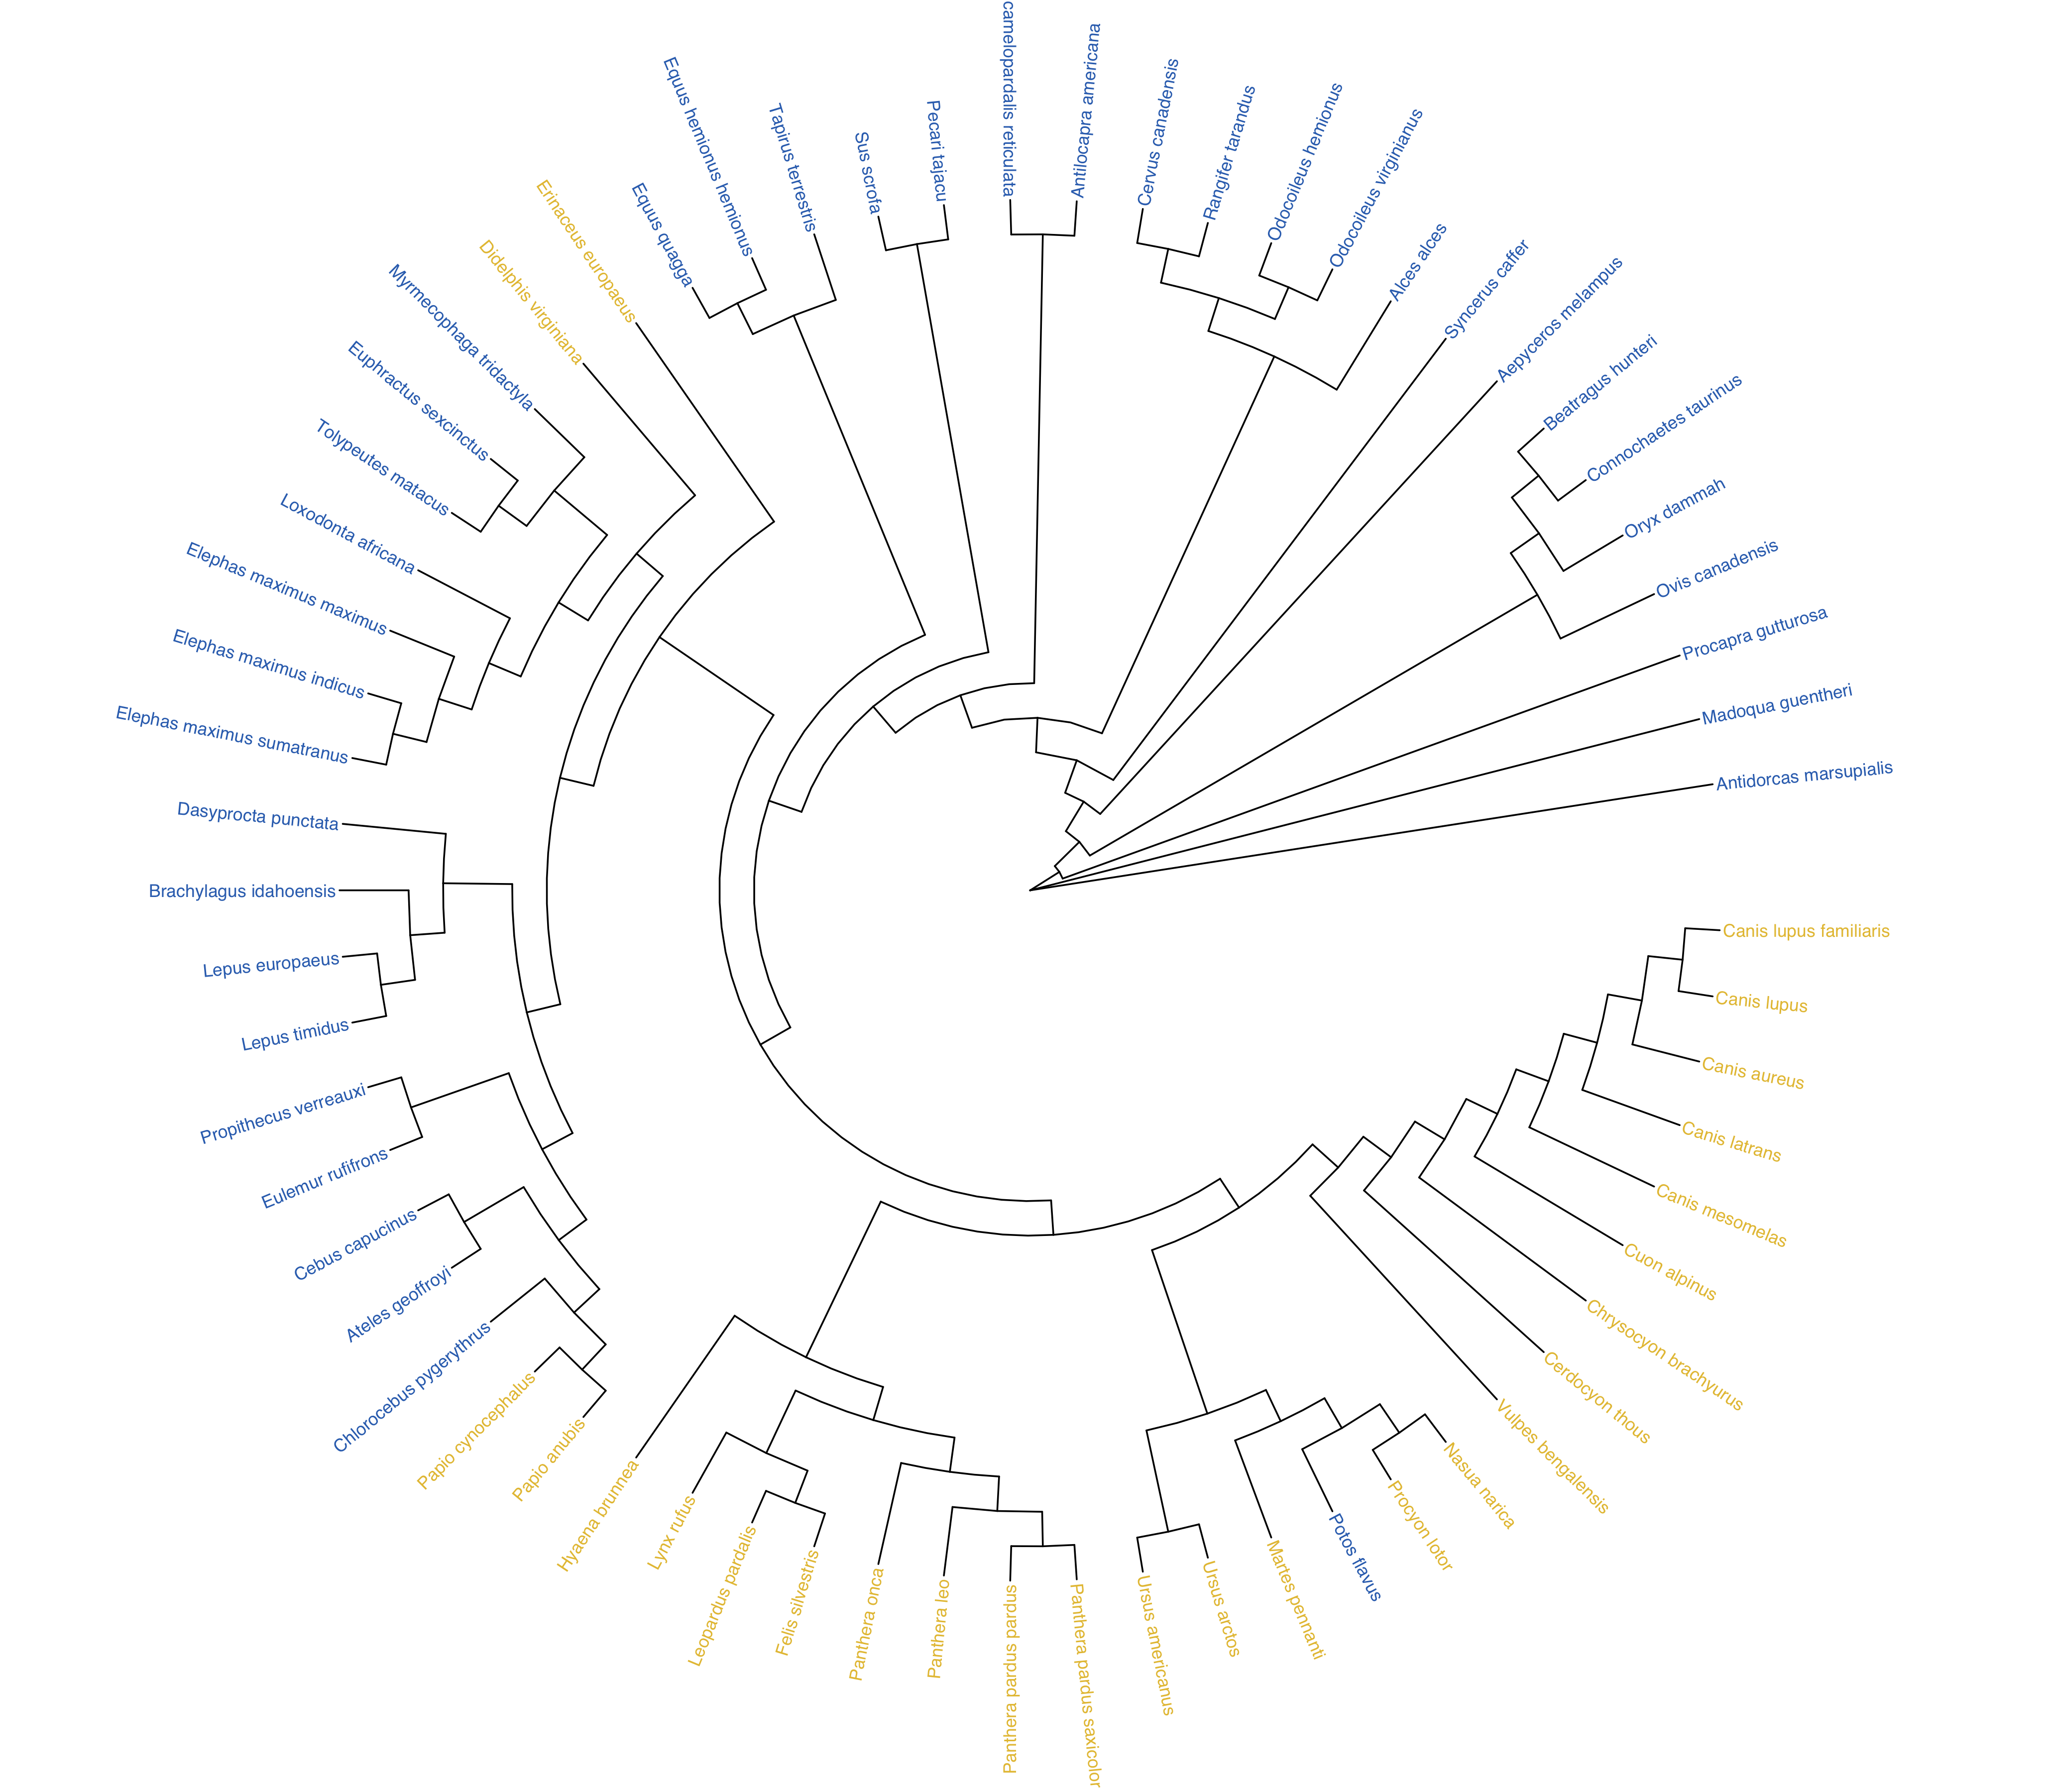
\includegraphics[scale=1]{Phylogeny.png}
%\caption{Phylogenetic relationships of the Mammalian species analysed in the main text.}
%\label{fig:phylogeny}
%\end{figure}

\begin{figure}[!h]
\centering
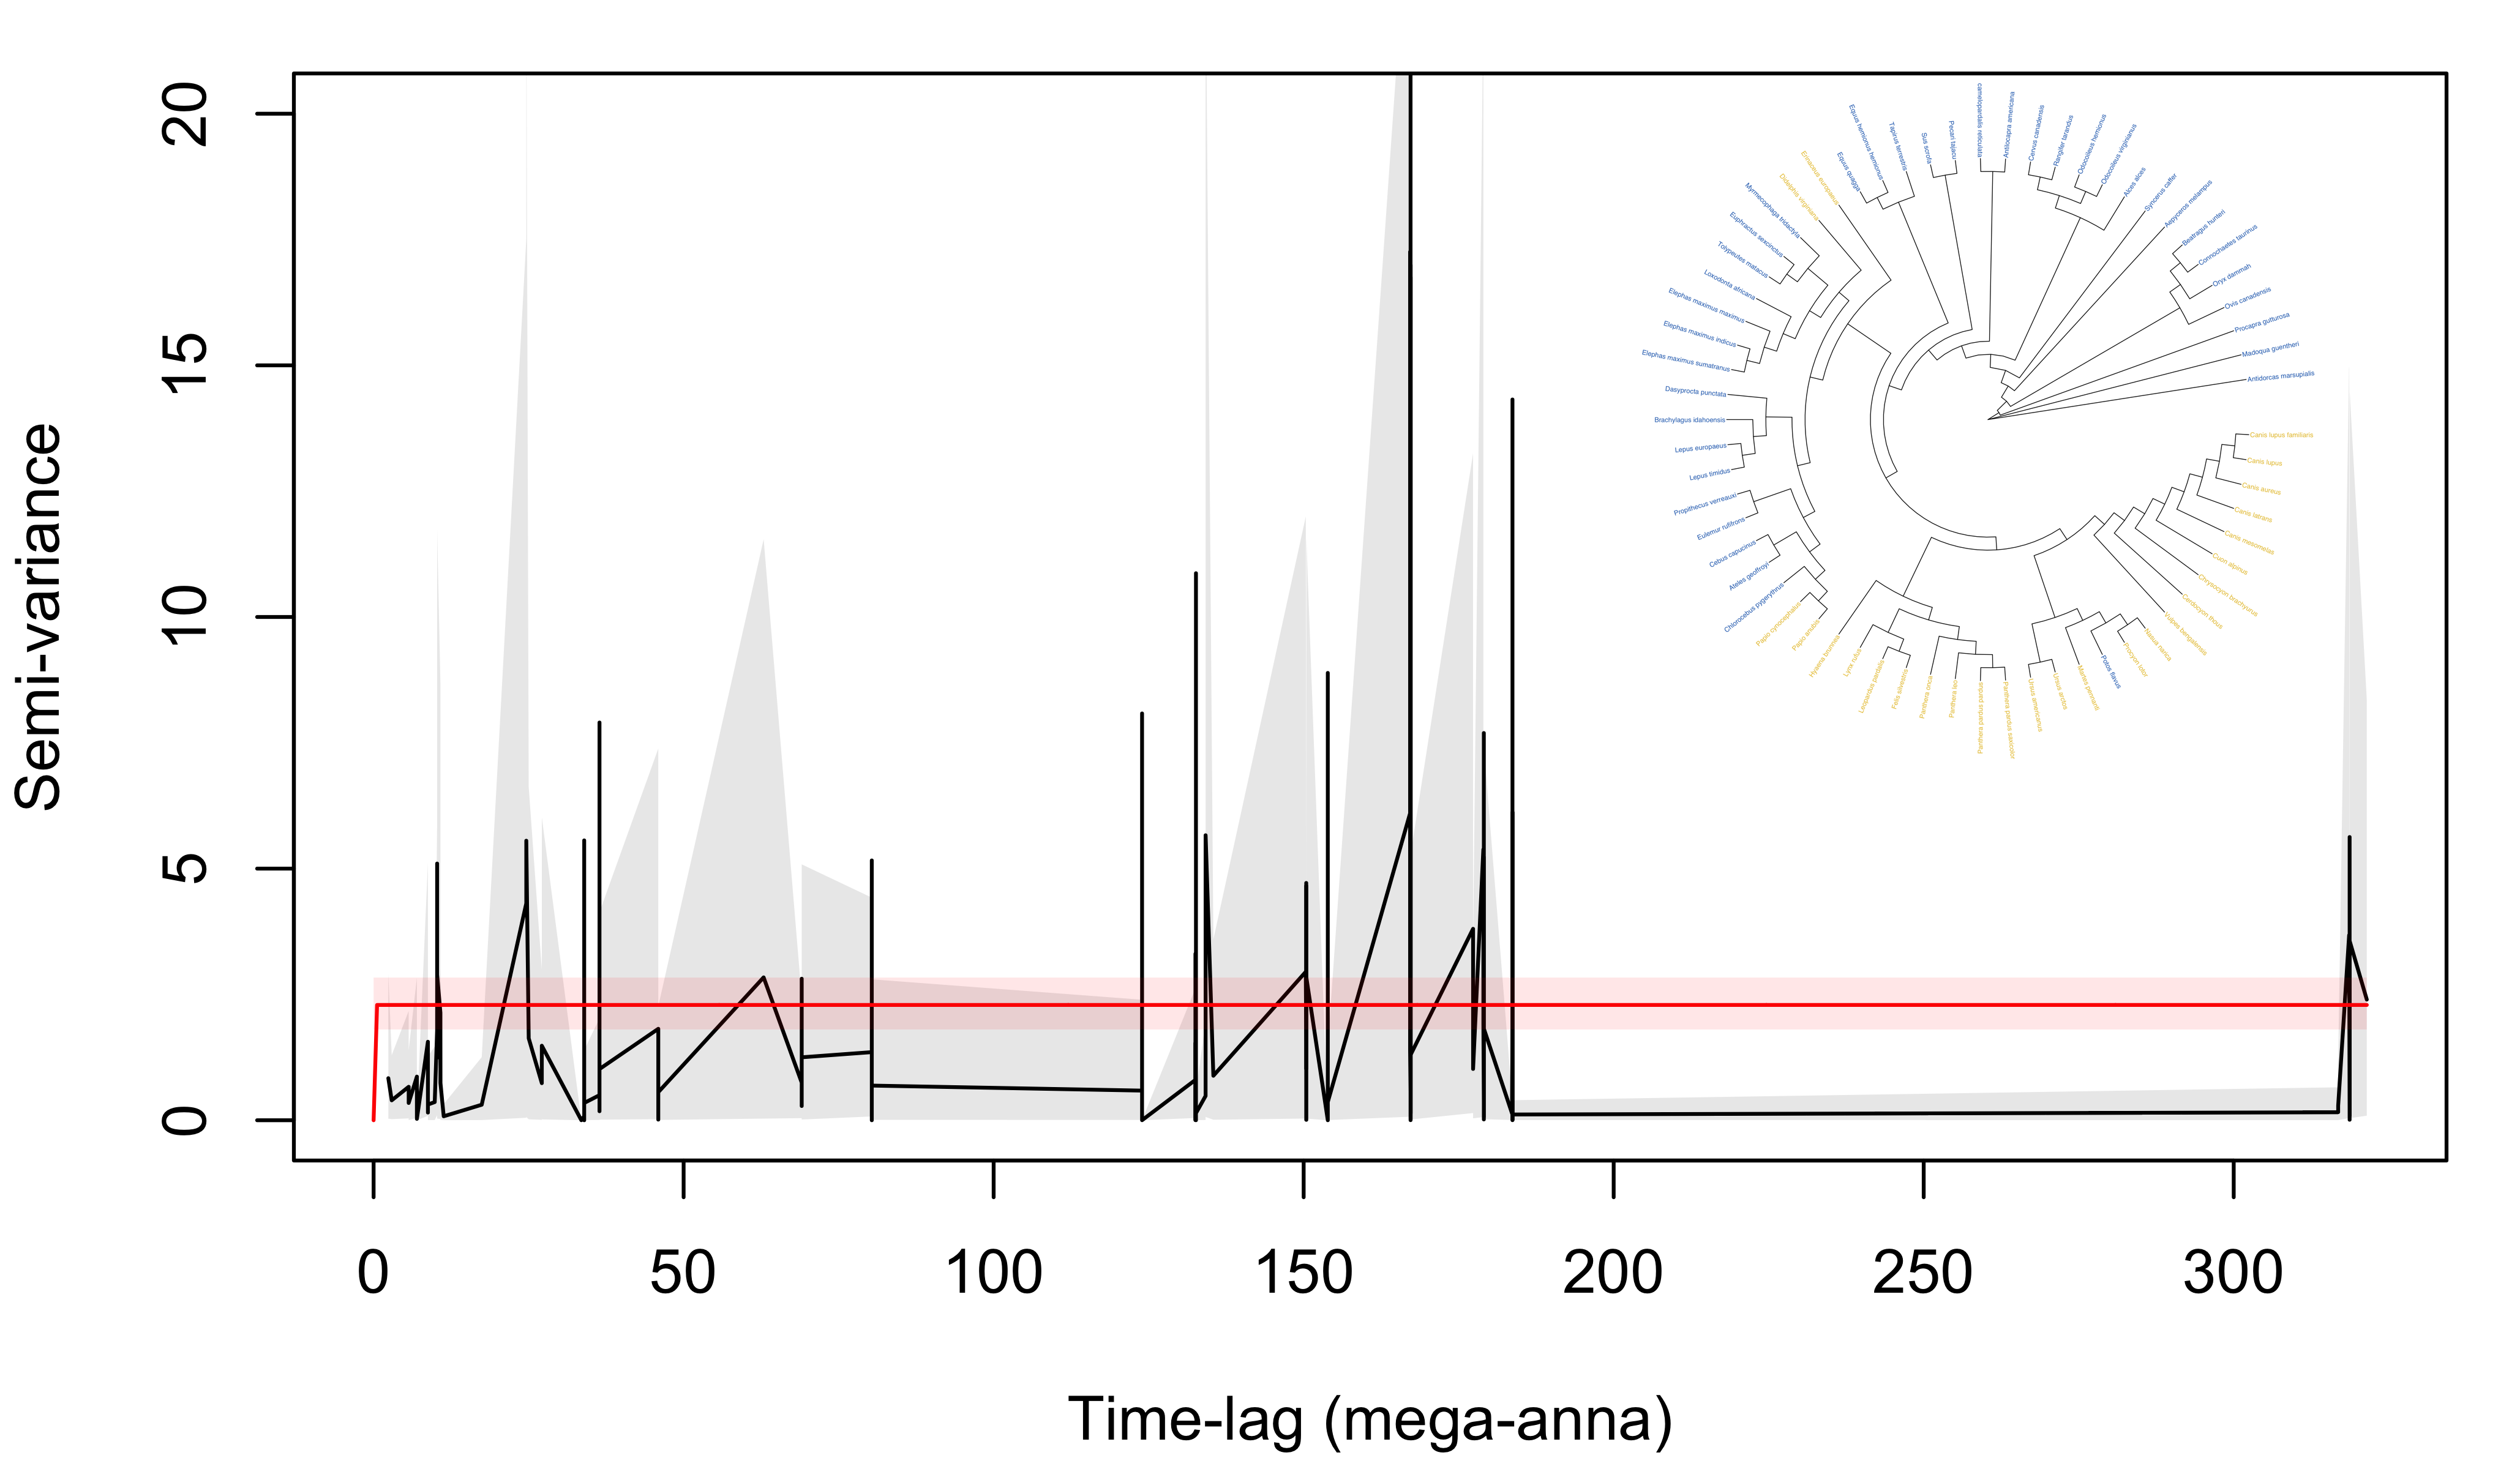
\includegraphics[scale=1]{Ballistic_Motion_SVF.png}
\caption{Empirical semi-variogram on Mammalian ballistic length scale. The black lines depict the estimated semi-variance at different time lags, wheres the grey shading show the 95\% confidence intervals. The red line and shading depict the estimated semi-variance under an Independent and Identically Distributed IID process. The inset shows the phylogenetic relationships of the Mammalian species analysed in the main text, coloured by dietary guild.}
\label{fig:SVF}
\end{figure}


Accordingly, we did not treat species data records as independent, but rather corrected for this inertia by including the phylogenetic relationships among species as a random effect in our allometric regressions. The phylogenetic relationships among species were included as a random effect in our allometric regressions using the \texttt{R} package \texttt{nlme} \cite{Pinheiro:2018}.



The final step in our analyses was to determine whether the stabilising selection around a mass invariant ration between predator and prey $l_v$ we found in our simulation study could also be observed in the empirical movement data. This required estimating the ratio of predator:prey $l_v$ for each species in our dataset. For this, we used the fitted allometric models described above to predict $l_v$ for the median body mass of each species' predators and prey. We then fit two models to these data, one that included a correlation with body mass, and an intercept only model. The relative support for these two models was then assessed using likelihood ratio tests.

%(SUPPLEMENTARY TABLE WITH MOD SELECTION RESULTS)

\end{document}

